%
% Hello! Here's how this works:
%
% You edit the source code here on the left, and the preview on the
% right shows you the result within a few seconds.
%
% Bookmark this page and share the URL with your co-authors. They can
% edit at the same time!
%
% You can upload figures, bibliographies, custom classes and
% styles using the files menu.
%
% If you're new to LaTeX, the wikibook at
% http://en.wikibooks.org/wiki/LaTeX
% is a great place to start, and there are some examples in this
% document, too.
%
% Enjoy!
%
\documentclass[12pt]{article}

\usepackage[english]{babel}
\usepackage[utf8x]{inputenc}
\usepackage{amsmath}
\usepackage{graphicx}
\usepackage[margin=0.75in]{geometry}
\usepackage{setspace}
\title{Multi-state RNAs and the cocktail party problem}
\author{Pablo Cordero, Wipapat Kladwang, Jeehyung Lee, and Rhiju Das}
\doublespacing
\begin{document}
\maketitle

\begin{abstract}
The ability of RNAs to undergo conformational changes is central to the various functions of many non-coding RNAs, ranging from gene regulation to protein synthesis. To fully grasp the nature of these changes it is necessary to understand the structural ensembles of these molecules at equilibrium. However, inferring RNA structural ensembles remains an open computational and experimental challenge. To address this problem, we present the RNA ensemble extraction from footprinting insights technique (REEFFIT), an algorithm that infers ensembles of secondary structures from multi-dimensional chemical mapping strategies, such as mutate-and-map (M$^2$) experiments. Inspired by the successes in blind source separation as metaphorized by the cocktail party problem, we developed REEFFIT as a factor analysis model that is able to robustly recover the underlying structural weights of noisy simulated M$^2$ data, without a set of structures given \textit{a priori}, as well as model the mutation-induced local perturbations corresponding to each state's contact map. The method can also extract the structure fractions in experimental capillary electrophoresis M$^2$ data of a bistable RNA hairpin that are in agreement with previous NMR estimates and account for the observed rearrangement patterns of the single-nucleotide mutants in M$^2$-seq signals for three other RNAs as read out by deep sequencing. These results establish REEEFIT and multi-dimensional chemical mapping methods, such as M$^2$, as a new and powerful approach to the RNA structural ensemble problem.
\end{abstract}

\section{Author Summary}

In the past decades, it has become clear that RNA is a versatile biological macromolecule that is heavily involved in gene expression, gene regulation, and structural scaffolding. Most of these roles rely on the ability of RNA molecules to self-assemble into intricate structures. However, it is an oversimplification to think that an RNA molecule folds just into one structure. Intense theoretical and experimental work has established that RNA is a dynamic structural entity that can adopt multiple conformations: an ensemble of structures that are present at equilibrium and may be of functional relevance. Although the computational study of RNA structural ensembles has become a classical subject in computational biology, the verification and dissection of these ensembles experimentally is still limited due to the size, resolution, and infrastructure constraints of state-of-the-art experimental methods such as magnetic resonance and X-ray scattering. We propose that coupling RNA chemical mapping or footprinting, an already widely used technique to probe RNA structure, to external perturbations, such as mutations in the case of mutate-and-map (M$^2$) experiments, can become a powerful experimental tool to probe ensembles at the single-nucleotide level. Inspired by the source separation problem in signal processing and aided by public chemical mapping data sources and current computational tools for natural-ocurring and synthetic riboswitches and ribozymes can fold into several states to detect a small molecule  \cite{Mandal2004,Winkler2003} catalyze a self-splicing reaction\ cite{Cate1996,Kennedy2013,Soukup1999}. These transitions depend on the affinity of each and every state in the RNA's structural ensemble to the external effector (e.g. ligand presence), as well as their respective equilibrium fractions \cite{Reining2013}. Probing these structural ensembles is therefore a key ingredient needed to understand the mechanisms of non-coding RNA \cite{Reining2013,Villordo2010}. 

From the computational viewpoint, structural ensembles have been thoroughly studied using the classic dynamic programming techniques devised in the past three decades \cite{McCaskill,Ding2005b}. However, the practical applications of  these methods have been mainly limited to refining minimum free energy secondary structure predictions. Although in theory bigger challenges such as riboswitch design and detection of pathogenic mutations can be addressed with these tools, the lack of experimental data that can validate the estimated structural ensembles undermines the confidence in the results. Indeed, there are few experimental techniques that can probe structural ensembles. State-of-the-art methods that can capture structural dynamics such as nuclear magnetic resonance (NMR) \cite{Bothe2011} and small angle X-ray scattering (SAXS) \cite{Russell2002,Wang2009} require costly infrastructure, focused technical expertise, and are limited to small RNA chains or lack nucleotide-level resolution. Chemical mapping or footprinting is a widely-used biochemical technique in which the RNA is exposed to chemical agents that modify unstructured parts of nucleic acids \cite{Mortimer2007,Tijerina2007}. These chemical modifications can be detected through a reverse transcription assay whose cDNA can be mapped back to the RNA sequence using electrophoretic separation or deep sequencing \cite{Mitra2008,Lucks2011}. Chemical mapping can probe molecules in solution at nucleotide resolution at least 200 nucleotides at a time, and has been used to probe entire viral genomes \cite{Wilkinson2008,Watts2009}. The ability to perform this technique in high-throughput allowed us to couple it with systematic mutagenesis: a mutate-and-map (M$^2$) strategy that can be used to infer the base-paring partners of each nucleotide in an RNA \cite{Kladwang2011,Kladwang2011f}. Intriguingly, we have observed that some single-nucleotide mutants have dramatically different chemical mapping profiles in all RNAs studied by M$^2$ to date, suggesting that these alternative states are prevalent throughout nature.

After proper quantification, chemical mapping yields a reactivity profile: one value per nucleotide correlated with how unstructured it is \cite{Mitra2008,Yoon2011}. If there are multiple conformations sampled by the RNA, the chemical reactivity profile can be seen as the linear combination of the structures present in the RNA's structural ensemble (Figure ~\ref{fig:statmodelfig}A). All the information about the ensemble is projected into the one-dimensional profile. Due to this projection, recovering the individual reactivity profiles for each state in the ensemble is impossible without further information. However, if the structural ensemble could be perturbed and remeasured enough times, we would then have enough data to estimate it. We can argue that this is exactly what is done in M$^2$ experiments: for the most part, each mutant's reactivity profile is the result of a different linear combination of the same structures present in the wild type (Figure ~\ref{fig:statmodelfig}B). The challenge to recover each state's reactivity profile and its weights can be cast as a source separation problem, a classical topic in signal processing \cite{Attias1999,Cardoso1998}. The source separation problem is best described by the "cocktail party" analogy \cite{Cardoso1998}. In the analogy, we are placed in a cocktail party with several people speaking at the same time and are challenged with finding the waveforms corresponding to the speech audio of each of the attendees, as well as their relative volumes, given audio recordings by microphones located in different corners of the room. When the number of microphones matches or exceeds the number of attendees, the mixed sources can be recovered robustly. Recovering RNA structural ensembles from chemical mapping data is analogous to this problem. Here, each attendee corresponds to a particular structure and each microphone recording to the observed reactivity profile of each mutant. Using this insight, we developed a method that models M$^2$ data as a linear combination of structures to estimate the structural ensembles of the wild type and all the single nucleotide mutants in the experiment. This analysis, which we have named RNA ensemble extraction from footprinting insights technique (REEFFIT), takes advantage of the variation in the reactivity profiles of each mutant caused by the stabilization and destabilization of structures in the ensembles induced by the mutation. 

REEFFIT uses a factor analysis framework to model the reactivity profile of each mutant in terms of the structures in the ensemble. To achieve this, REEFFIT finds both the expected reactivity profile of each structure and a convex combination of weights that best model the data. In case the set of structures contained in the ensemble is not known \textit{a priori}, REEFFIT makes an educated guess by clustering the suboptimal structures predicted for the mutants, picking the best representative of each cluster given the data, and subsequently adding more structures that would increase the value of a likelihood-based information score. REEFFIT also estimates the per-experiment noise levels and models local perturbations induced by, e.g., mutations.

Because of its underlying general factor analysis framework, REEFFIT is easily extensible and provides a basis for future modeling of chemical mapping data. Importantly, REEFFIT is not limited to M$^2$ experiments: the only requirements are that all reactivity profiles in the dataset are perturbed versions of approximately the same ensemble of structures and that the number of profiles is at least as large as the number of the most prevalent structures in the ensemble. It is therefore theoretically possible to use sources of perturbations other than mutations such as changing ionic concentrations  \cite{Das2010}, temperature, or concentration of small molecule binders \cite{Kladwang2011f}, or macromolecule partners \cite{Kladwang2010}.

We give a detailed description of the statistical framework and technique below. We validate our method using simulated and experimental data. We finally discuss potential applications and future improvements. 


\section{Results}
\subsection{The REEFFIT statistical model}
Given a set $S =  \{ S_1, S_2, …, S_{t} \}$ of secondary structures with reactivity profiles $D = \{ D_{1}, D_{2}, ..., D_{t} \}$ , REEFFIT models the observed reactivity profiles, $D^{obs}$ as linear, convex combinations of the reactivity profiles of $D$ plus white noise (see Figure ~\ref{fig:statmodelfig}B). $D$ is a set of hidden variables since we do not know what the isolated reactivity profiles of each structure are. However, we can impose a prior on each of these hidden profiles depending on their secondary structures. Each $D_{s}$ can be decomposed into a set of univariate random variables $D_{si}$, one for each nucleotide $i = 1, 2, ..., n$, where $n$ is the number of nucleotides (here and throughout the text, $D$ will be treated as a $m \times n$ matrix, with rows denoted as $D_{s}$ and columns as $D_{i}$, where $s$ is a structure index and $i$ is a position index). Because low and high chemical reactivities are correlated with structured and unstructured states, a reasonable prior would force $D_{si}$ to be small if $i$ is paired in structure $S_s$ and higher if it is unpaired. To get distributions of the reactivities of paired and unpaired nucleotides, we compiled all the SHAPE reactivity data in the RNA Mapping Database (RMDB) \cite{Cordero2012} of RNAs with known crystallographic structure and modeled it in terms of mixtures of gamma distributions as described previously \cite{Cordero2012a}. Let $RMDB_U$ and $RMDB_P$ be the modeled RMDB unpaired and paired distributions respectively, we can then define a prior likelihood for $D_{s}$ as: 
\begin{align}
  &\begin{aligned}
RMDB_{s}(x) &= \prod_i (RMDB_U(x) \mbox{I}\left[i \mbox{ is paired in } S_s\right]\\ 
                &+ RMDB_P(x) \mbox{I}\left[i \mbox{ is unpaired in } S_s\right])
  \end{aligned}
\end{align}

where $\mbox{I}$ is the indicator function. Because these distributions were estimated using SHAPE data, any statistical model based on them will only work properly in SHAPE-based chemical mapping experiments. To handle other modifiers, e.g. dimethyl sulfate (DMS), $RMDB_P$ and $RMDB_U$ would be replaced with the respective estimated distributions using unpaired and paired data of that modifier \cite{Cordero2012a}. After defining our priors for each structure profile, we can write the REEFFIT model (see also Figure ~\ref{fig:statmodelfig}):

\begin{align}
  &\begin{aligned}\label{reeffit_model}
    D^{obs}_{i} &= WD_{i} + \epsilon_{i}\\
    D_{s} &\sim RMDB_{s} \\
    \epsilon_{i} &\sim \mathcal{N}(0, \Psi_{i}I_{m}) \\
    \sum_{s}^{t} W_{js} &= 1, \forall j = 1, …, m\\
  \end{aligned}
\end{align}


Here, $D^{obs}_{i}$ and $D_{i}$ are the column vectors of $D$ indexed by nucleotide position, $W_{js}$ is the weight for the profile of structure $s$ in the observed profile $j = 1 , 2, ..., m$ with $m$ the number of mapping profiles in the experiment, and $\epsilon_{i}$ is centered white noise with a diagonal covariance matrix $\Psi_{i}I_{m} \in \Re^{m \times m}$ where $\Psi_{i}$ is a scalar and $I_{m}$ is the identity matrix of $\Re^{m \times m}$. Our model differs from the standard factor analysis model \cite{Ghahramani1996} in two ways. First, we have $n$ rather than one $\epsilon$ variable to capture experimental noise. This derives from our observations that different sequence positions have widely different experimental error distributions depending on the intensity of the reactivity and proximity to the beginning and end of the sequence \cite{Kladwang2011}. Second, different sequence positions are assigned different prior distributions that depend on the pairing state of each structure in the model. It is important to note that here, as in standard factor analysis, all covariance matrices for the noise must be diagonal, that is, the measurements are independent of each other \cite{Ghahramani1996,Rubin1982}. This assumption holds in the case of multiple chemical mapping measurements, since each measurement does not affect the others in any way.

There is no closed form maximum likelihood estimation for this model and therefore an expectation maximization (EM) algorithm is typically used to obtain expected values for the hidden variables (in our case, $D$), and maximum likelihood estimates for $W$ \cite{Ghahramani1996,Rubin1982}. In standard factor analysis, the E-step can be obtained in closed form by calculating the sufficient statistics for the likelihood function, which happen to be the first two moments of the posterior distribution of $D$: $E[D | D^{obs}]$ and $E[DD^T | D^{obs}]$. Unfortunately, the extremely non-gaussian form our priors for each $D_{s}$ precludes us from having a closed form for these statistics and we must calculate them using Markov Chain Monte Carlo (MCMC) [see Materials and Methods]. For the M-step, closed form solutions depending on these sufficient statistics exist for $W$. Additionaly, we incorporate convex combination constraints on $W$ by casting it as a quadratic problem and solving numerically (see Materials and Methods).

\subsection{Selecting the structures for the model}
Most of the time it is not clear \textit{a priori} what set of structures would best model the data. To select a good starting set of structures, we can calculate a set of suboptimal structures for each mutant in the M$^2$ experiment. We then proceed to cluster the structures using hierarchical clustering with a probabilistic distance metric and a Calinski-Barabasz cutoff (see Materials and Methods and Figure ~\ref{fig:structselectfig}A). Taking the structures in ensembles of all mutants allows for a broader search of structures than may be needed in to fully explain the data. We select structure medoids for each cluster by taking the one that is found to be most stabilized by any of the mutants. Finally, structures may randomly added in a greedy manner by maximizing the Akaike information criterion which penalizes model complexity to avoid overfitting \cite{Akaike1987} (see Materials and Methods and Figure ~\ref{fig:structselectfig}B).


\subsection{Simulated data evaluations: an \textit{in silico} benchmark}
To first evaluate REEFFIT, we tested if it could recover the structures and ensemble weights used to simulate a benchmark of short representative RNA sequences for 20 Rfam families \cite{Gardner2011} that include microRNAs, small nucleolar RNAs, and viral sequences. We simulated M$^2$ chemical mapping data using small sets of structures in the suboptimal ensemble of each RNA (see Materials and Methods). We then ran our structure set selection algorithm and fitted model ~\ref{reeffit_model} to the simulated data. Evaluating REEFFIT's performance is challenging since we have to somehow compare the weights of the predicted and data-generating structures and at the same time assess the model's goodness of fit to the data. Therefore, we chose to evaluate REEFFIT's predictions using several metrics. 

First, we compared the structures that REEFFIT inferred to the ones used to generate the data. Because REEFFIT uses a conservative information score to obtain a set of structures to model the data, in many cases it inferred less structures than those used to generate the data. In these cases (such as the RF00436 sequence, see Figure ~\ref{fig:insilicofig}) the generating structures are too similar to each other and can be accounted for by taking just one of the structures as a representative. Because REEFFIT infers the structures by clustering, we can compare the weights of these extra generating structures to our predicted ones by grouping them in REEFFIT's clusters. Therefore, instead of comparing predicted to original structures, we compare predicted structures to original clusters. Each cluster weight is then defined to be the sum of the weights of all the structures in each cluster (see Figure ~\ref{fig:insilicofig}A and ~\ref{fig:insilicofig}B). A similar evaluation scheme can be taken in the very rare case when the predicted structures are more than the generating structures, (such as RF00108, see Table ~\ref{insilicobenchmark}). In these cases we compare predicted structures with clusters of generating structures. In the same way as before, the weight for each cluster is the sum of the weights of the generating structures in that cluster. Using this validation scheme, REEFFIT is able to recover the weights within error most of the time (see Table ~\ref{insilicobenchmark}).

Second, we assesed the goodness of fit of the model. Goodness of fit metrics for factor analysis have been extensively studied in psychometrics under the umbrella of structural equation modelling \cite{Schreiber2006,Marsh1988,Babyak2010}. In line with these studies, we report $\chi^2/df$ and root mean square error of approximation (RMSEA) as goodness of fit metrics for the fitted models to each simulated dataset. The general low RMSEA values and $chi^2/df$ indicated that the structures proposed by REEFFIT fit the data well: only the RF00108 sequence, the only case that was modeled with more structures than it was generated with, gave a $\chi^2/df$ value over 2.    

\subsection{Experimental evaluation using deep sequencing}

We proceeded to test REEFFIT with experimental data. We tested our method using chemical mapping data read out with capillary electrophoresis and deep sequencing platforms. To test our method using deep sequencing, we obtained M$^2$-seq measurements for a benchmark of three RNA sequences of our own design using the EteRNA expert interface (see Materials and Methods): the MedLoop, MedLoop$\Delta$, and M-stable RNAs. We have previously studied the MedLoop RNA in a proof-of-concept test case for the M$^2$ methodology \cite{Kladwang2011}. The wild type MedLoop forms a stable 10 base-pair hairpin while some mutations that disrupt that helix force it into an alternative stem (see Figure ~\ref{fig:medloopfig}A). According to REEFFIT, the MedLoop M$^2$ data can be modeled with these two structures: a 10-base pair helix (which we will denote by $mlp_1$) and an alternative 3' hairpin ($mlp_2$). As expected, $mlp_1$ (Figure ~\ref{fig:medloopfig}A,  blue) is the predominant state in most of the constructs, including the wild type sequence, while $mlp_2$ (green) becomes dominant when the $mlp_1$ helix is destabilized by mutation. Interestingly, mutations in the loop of $mlp_1$, such G11C and A17U, seem to destabilize the structure, resulting in a mixture of the two states. Furthermore, mutating the 5' part of the $mlp_1$ helix results in more destabilization of the structure than mutating the 3' side (compare the weights of each structure e.g. A5U to U31A). This is expected since the helices of $mlp_1$ and $mlp_2$ share the 3' range of nucleotides for that helix (G26 to G34); mutating these residues destabilizes $mlp_1$ but produces a weaker version of $mlp_2$, resulting in a mixture of states. 

The MedLoop$\Delta$ construct differs from MedLoop in that it lacks five nucleotides in the 3' end, which abolishes the alternative stem. REEFFIT models the MedLoop$\Delta$ M$^2$ data with three structures: $mlp_1$ (blue in Figure ~\ref{fig:medloopdeltafig}A, same structure as $mlp_1$ for the MedLoop RNA), $mlp_1'$ (green), and $mlp_3$ (red). The $mlp_1'$ structures is a variation  of the $mlp_1$ structure of the MedLoop RNA: $mlp_1'$ has an extra helix that is made possible by the 5-nucleotide deletion. In the wild type sequence, $mlp_1$ is the main structure with a predicted mean weight of 1. Across the rest of the mutants, $mlp_1$ and $mlp_1'$ alternate as the dominant structure. When the main helix of $mlp_1$ and $mlp_1'$ is destabilized (e.g. in the C3G mutant, see also the I and II features marked in Figure ~\ref{fig:medloopdeltafig}), $mlp_3$ appears in the structural ensemble, but it is never stabilized beyond a weight of 0.5. 

The final M$^2$-seq test case was the M-stable construct, an RNA whose minimum free energy structure is predicted to be a simple hairpin with a tetraloop (see orange structure, Figure  ~\ref{fig:medloopdeltafig}A, which we will denote as $mst_1$). The structure is deceptively simple: the structural ensemble of the construct is predicted to have at least 2 other structures 1 kcal away from the $mst_1$. This unstable ensemble is susceptible to change drastically by mutation and therefore presents a challenging case for REEFFIT. The M$^2$-seq measurements clearly indicate the presence of more than three structures when all the mutants are taken into account. REEFFIT models the M-stable data with 4 states (see Figure ~\ref{fig:medloopdeltafig}A). Interestingly, each alternative structure (blue, green, and red; denoted as $mst_2$, $mst_3$, and $mst_4$, respectively) has at least one non-cannonical base pair -- each of these structures were found in the set of suboptimal structures of a mutant. Nevertheless, REEFFIT can model the data well with these four states. Weights for the wild type include structures $mst_2$ and $mst_3$. In particular, $mst_2$ is predicted to be as stable as $mst_1$. These two structures share the same hairpin, but structure $mst_2$ has two helices surrounding it, separated by a G10 bulge. Evidence for $mst_2$ in the wild type profile can be seen in nucleotides A8 to C14 and G39 to A45, where the extra helices of $mst_2$ partially protect those residues. Structure $mst_3$ also appears in the wild type ensemble, but only in a 0.15 fration -- the only evidence of its presence in the wild type profile being the increased reactivity at positions A30, A31 and U44, A45. In the rest of the mutants, these structures change weights drastically, but $mst_1$ and $mst_2$ maintain dominance as made evident by the only punctate feature of the data: the cross-diagonal pattern of the shared helix of $mst_1$ and $mst_2$.


\subsection{Experimental evaluation using capillary electrophoresis}

Previously, Hobartner and colleagues used imino proton NMR spectra to estimate the ensemble weights of two structures in a bistable RNA hairpin (Figure ~\ref{fig:hobartnerfig}A) \cite{Hobartner2003}. The simplicity of this system allowed the authors to decompose its NH...N 1H NMR spectrum into a weighted sum of the NMR spectra of each hairpin without the need of resonance assignment and therefore presents an excellent test case for REEFFIT. We synthesized this RNA and obtained M$^2$ measurements for this system using capillary electrophoresis as a read-out (see Materials and Methods). Visual inspection of the reactivity profile for the wild type and the global rearrangements occurring in most mutants hint of the bistable nature of this RNA (Figure ~\ref{fig:hobartnerfig}C). Unless perturbed, this bistable RNA folds predominantly into a haripin with its helix in the 3' end (blue structure in Figure ~\ref{fig:hobartnerfig}), which we will denote as $hob_1$. When the $hob_1$ helix is perturbed by mutation, the RNA switches to a 5' helix structure (green, denoted here as $hob_2$). Some constructs in this M$^2$ experiment, e.g. G8C, have a mixture of these two structures in their ensembles. As in the MedLoop M$^2$ data, the two states share a region of nucleotides in their respective helices (G11 to U13) and therefore the mutations have asymmetrical effects: mutations affecting this region have little effect in the ensemble since they destabilize both structures, while more 3' mutations destabilize $hob_1$ significantly. the mutations have asymmetrical effects. The wild type RNA is a mixture of these two states, $hob_1$ is present 70\% of the time and $hob_2$ 30\%. These estimated weights are in agreement with the previously reported fractions by Hobartner et al. (Figure ~\ref{fig:hobartnerfig}B). Furthermore, combining the profiles of U4A and C23G, mutants that are predicted by REEFFIT to stabilize $hob_1$ and $hob_2$ respectively, result in a profile that follows closely the wild type reactivities (Figure ~\ref{fig:hobartnervalidationfig}).

\section{Discussion}

Probing the structural ensembles of RNA molecules is a formidable task that is essential to understand their thermodynamics and can give important insights in their biological functions \cite{Bothe2011}. Current experimental techniques used to probe these ensembles require significant infrastructure investment, technical expertise, and are limited to small RNA sequences. We presented a novel strategy based on easily obtainable chemical mapping measurements that can be used to address this challenge. By taking advantage of the ensemble perturbations induced by single-nucleotide mutations in M$^2$ experiments, we have cast the RNA structural ensemble challenge as a source separation "cocktail party" problem \cite{Cardoso1998}. The resulting algorithm that solves this problem, REEFFIT, extracts structural ensembles out of multi-dimenwsional chemical mapping experiments. Although we have evaluated our method using M$^2$ measurements, REEFFIT can also be used to analyze other multi-dimensional chemical mapping experiments where the source of perturbation is other than mutation. 

For M$^2$ experiments, REEFFIT can be used to tease out the observed changes due to structural ensemble perturbations and the local perturbations induced by the mutations themselves. This enables extracting additional insights from this information-rich strategy and helps deconvolute global structural rearrangements and the embedded “contact map” of the RNA that we have previously used to refine secondary structure predictions \cite{Kladwang2011f}.

REEFFIT's statistical model can be easily extended to use different priors for the structure reactivity profiles due to the use of MCMC. For example, instead of classifying nucleotides in paired and unpaired states, we could group them by secondary structure element (hairpin, edge base-pair, bulges, interior loops, etc.) and assign different reactivity distributions for each element, analogous to what we have done to calculate $RMDB_U$ and $RMDB_P$. In fact, following this rationale, it would also be possible to obtain three-dimensional ensembles using an appropriate structure space sampling scheme \cite{Frellsen2009,Das2007,Das2010,Jonikas2009}. This may become a reality in the near future as we obtain enough chemical mapping measurements in order to robustly estimate the prior distributions of each three-dimensional structure motif.

We expect REEFFIT to be used routinely to analyze multi-dimensional mapping experiments, not only to dissect the complex ensembles of various biologically-relevant molecules such as the structure fractions of riboswitches in the absence of ligand, but to detect systematic flaws in current secondary structure energy functions and provide insights for the design of RNA circuitry. The commoditization of sequencing technologies will further expand the use of RNA chemical mapping for structure probing and REEFFIT will help in the dissection of these data and push forward a view of that includes experimental probing of structure thermodynamics that goes beyond the implicit dogma of "one sequence, one structure". 



\section{Materials and Methods}

\subsection{Maximum likelihood estimation of the REEFFIT model}
Given the REFFIT factor analysis model (\ref{reeffit_model}) we want to calculate maximum likelihood estimates for $W$ and each $\Psi_{i}$ given the hidden variables $D$. We will use an expectation maximization (EM) algorithm to calculate these maximum likelihood estimates given expected values of the hidden variables. Let $R = -\frac{nm}{2}\log(2\pi)$, then the log-likelihood function $L$ can be written as:

\begin{align}
  &\begin{aligned}
    L(W, \Psi) &= \sum_i^n \log \frac{1}{(2\pi)^{m/2})^T|\Psi|^{1/2}} \exp(-1/2(D^{obs}_i - WD_{i}) 1/\Psi I_{m}(D^{obs}_i - WD_{i})) \\
               &=  R -\frac{1}{2}\sum^n_i -\log|\Psi_{i}I_{m}| + ((D^{obs}_i)^T 1/\Psi I_{m} D^{obs}_i - 2(D^{obs}_i)^T 1/\Psi I_{m} W D_{i} + D_{i}^TW^T 1/\Psi_{i} I_{m} W D_{i})\\
               &= R -\frac{1}{2}\sum^n_i -m\log(\Psi_{i})	 +  ((D^{obs}_i)^T 1/\Psi_{i}I_{m} D^{obs}_i - 2(D^{obs}_i)^T 1/\Psi_{i}I_{m} W D_{i} + Tr[W^T 1/\Psi_{i}I_{m} W D_{i}D_{i}^T])\\
   \end{aligned}
\end{align}

, where $Tr[.]$ is the trace operator. For the E-step, we take the expectation of $L$ conditioning the hidden variables $D$ with respect to the data:

\begin{align}
  &\begin{aligned}
    E[L| D^{obs}] &=  R -\frac{1}{2}\sum^n_i -m\log(\Psi_{i})	 + ((D^{obs}_i)^T1/\Psi_{i}I_{m}D^{obs}_i - 2(D^{obs}_i)^T 1/\Psi_{i}I_{m} WE[D_{i}|D^{obs}_i]\\ 
    & + Tr[W^T 1/\Psi_{i}I_{m} WE[D_{i}D_{i}^T|D^{obs}_i])\\
   \end{aligned}
\end{align}

We thus have that the sufficient statistics of $L$ are the first two moments of the posterior distribution of $D$: $E[D_S | D^{obs}]$ and $E[DD^T | D^{obs}]$. Because of the forms of our priors (mixtures of gamma distributions, see \cite{Cordero2012a}), these sufficient statistics cannot be written in closed form. We therefore estimate them using a Markov Chain Monte Carlo algorithm with an adaptive step rule implemented in the pymc python library for bayesian statistics \cite{Patil2010}. MCMC can be computationally expensive, especially when used in combination with EM. Because we are assuming no positional correlation between reactivities, the MCMC simulations can be performed independently. Therefore, in our implementation we parallelize these position-wise MCMC calculations using the python joblib parallelization library.\\
For the M-step, given the sufficient statistics above, we calculate $W$ by maximizing $L$ with respect each variable, enforcing the convex combination constraints in (\ref{reeffit_model}). We can cast the minimization of $L$ with respect to $W$ as a quadratic program;	 let $W_j$ be the $j$-th column of $W$, indexed by measurement/mutant, then for each chemical mapping measurement $j$:


\begin{align}
  &\begin{aligned}\label{W_qp}
   \mbox{minimize } &(\sum_i^n \frac{1}{2\Psi_{i}})W_j^TE[D_SD_S^T | D^{obs}]W_j - (1/\Psi_{i}I_{m}(\sum_i^n D^{obs}_{ji}E[D_S | D^{obs}]_i))^TW_j\\
   \mbox{subject to } & \sum_{s}^{t} W_{js} = 1, \forall j = 1, …, m
   \end{aligned}
\end{align}
 
To calculate $W$, we solve the resulting quadratic programs using the CVXOPT python library \cite{Dahl2006}. In standard factor analysis the single noise covariance matrix is re-estimated in each EM iteration. However, because we have different covariance matrices for each sequence position, we are underpowered to estimate these from the data. We therefore do not re-estimate each $\Psi_{i}$ and maintain its initial value.

%After obtaining $W$ we can calculate $\Psi$ using the standard factor analysis solution:
% \begin{align}
%  &\begin{aligned}
%    \Psi = \frac{1}{n}\mbox{diag}\left[\sum^n_i %D^{obs}_i(D^{obs}_i)^T - 2(\sum^n_i D^{obs}_iE[D_{i}|%D^{obs}_i]^T)W^T + W(E[D_{i}D_{i}^T | D^{obs}_i])W^T\right]
%   \end{aligned}
%\end{align}

where $\mbox{diag}[.]$ is the diagonal operator to constrain $\Psi$ to be a diagonal matrix. The final estimates of $W$, $\Psi$, and the expected reactivities $E[D_S|D^{obs}]$ are calculated until the value for $L$ is stabilized and does not substantially improve.\\

Because of the hidden reactivities $D_S$, $L$ need not be convex and may have multiple local maxima. The EM algorithm simply reports one of these local maxima and is therefore sensitive to initial conditions. For each $\Psi_{i}$ we choose the empirical variance of position $i$ across all chemical mapping measurements, consistent with the variance calculation performed when using M$^2$ z-scores as pseudo-energy bonuses for secondary structure prediction \cite{Kladwang2011f}. For $W$, we use the dynamic programming algorithm in RNAstructure to calculate the energies of each structure in each mutant. For mutant $j$, let $\Delta G_{js}$ be the RNAstructure-calculated energy for structure $i$, $k_B$ the Boltzmann constant, and $T$ the temperature at which the experiments were performed, then the initial value $W_0$ at position $(j,s)$ is:
\[W_{0,js} = \frac{\exp(-\Delta G_{js}/(k_BT)}{\sum_{s'} \exp(\Delta G_{js'}/(k_BT))}\]

To calculate uncertainties for $W$, we use a Fisher's information matrix approach. Usually, the information matrix for $W$ would take the form:

\[\mathcal{I}(W) = -E\left[\frac{\partial^2 L}{\partial W^2} \mid W\right]\]

For expectation maximization, in the case of hidden variables, it has been shown that $\mathcal{I}$ can be estimated as follows \cite{Oakes1999}:

\[\mathcal{I}(W) = -\frac{\partial^2 E[L| D^{obs}]}{\partial W^2}\mid_{W=W^*}\]
 
with $W^*$ the maximum likelihood estimate obtained from the EM algorithm. Throughout this paper, we report uncertainties for $W$ in the form of $\sigma_W = \frac{1}{\sqrt{\mathcal{I}(W)}}$. Uncertainties for the expected reactivity profiles, $E[D_S|D^{obs}]$, are reported as standard errors resulting from the MCMC simulations:

\[SE_{D_{i}} = \frac{\sigma_{D_{i}}}{\sqrt{nsim}}\]

Here, $\sigma_{D_{s}}$ is the sample standard deviation from the MCMC trace for the reactivity values of $s$ at sequence position $i$ and $nsim$ is the number of samples used in the simulation calculations. Finally, uncertainties for the predicted data $W^*E[D|D^{obs}]$ are calculated by propagating the uncertainties $\mathcal{I}(W)$ and $SE_{D_{i}}^2$.

\subsection{Handling local perturbations}

Systematic experimental perturbations used to alter the RNA's structural ensemble may induce local changes that cannot be captured by the linear combination of the weights $W$ and the expected reactivities $E[D|D^{obs}]$. This is the case in M$^2$ experiments, where mutations induce local perturbations in the underlying reactivities of each structure. To model these perturbations, we add a set of random variables to our model: $C = \{ C_{sji} \}$ for all structure $s$, mutant $j$, and sequence position $i$ where $i$ is at most one nucleotide away from the site of a mutation in mutant $j$ or from a base pair that would be disrupted in structure $s$ in mutant $j$. These variables take the values of the change in reactivity of $D_S$ at perturbed positions that are needed to account for the data. We include $C$ in the MCMC calculations used to estimate the sufficient statistics, setting their prior distribution to the distribution of differences in reactivities in M$^2$ experiments available in the RMDB, which we call $RMDB_{\Delta}$ and that we model with a Laplace distribution. The MCMC simulations yield the expected values of $C$ given the data: $E[C|D^{obs}]$. In all likelihood calculations and in the quadratic problem for $W$ (\ref{W_qp}) we incorporate $E[C|D^{obs}]$ by adding $E[C_{sji}|D^{obs}]$ to  $E[D_{si}|D^{obs}]$ in the relevant operations involving mutant $j$.

\subsection{Marking missed data points}
To detect where our model fails to predict observed values we use the estimated noise levels in $\Psi$. For each data point $D^{obs}_{ij}$ we can calculate its probability given our model: 

\[P(D^{obs}_{ij} \mid W,\Psi,E[D_S|D^{obs}]) = \mathcal{N}(WE[D_S|D^{obs}]_{ij},\Psi_{ii})\]

Any data point whose probability given our model is below 0.05 is marked as missed (see Figures ~\ref{fig:synthetichairpinfig}, ~\ref{fig:hobartnerfig}, and ~\ref{fig:medloopfig}, red squares).

\subsection{Initial structure set selection procedure}

When a set of structures is not provided \textit{a priori}, REEFFIT draws a subset of structures from the suboptimal structures of all sequences in the experiments that would best model the data. In M$^2$ experiments, the suboptimal structures of all mutants involved are taken into account. Theoretically, to find the best structures that model the data we could enumerate all possible combinations of structures, fit model (\ref{reeffit_model}) to each combination, calculate some penalized information score, and choose the combination with the best score. In practice, this method is intractable for a large set of structures due to the exponential number of combinations of structures. Furthermore, the quadratic nature of the likelihood function does not allow a nested decomposition required for search space reduction techniques such as dynamic programming. Instead, we choose to explore structures that are most representative of the combined set of suboptimal structures. To achieve this, we perform hierarchical clustering using a distance metric that takes into account the position-wise \textit{a priori} reactivity distributions of each structure $S_s$ (in our case, either $RMDB_U$ or $RMDB_P$). For a nucleotide position $i$, let the probability distribution $RMDB_{S_{is}}(x) = RMDB_U(x) I\left[i \mbox{ is paired in } S_s\right] + RMDB_P(x) I\left[i \mbox{ is unpaired in } S_s\right]$, and $JS$ the Jensen-Shannon distance between distributions; we define the following distance metric:

\[d(S_s, S_r) = \sum^n_i JS(RMDB_{S_{si}}, RMDB_{S_{ri}})\]

Performing hierarchical clustering using $d$ as our metric of choice clusters the structures given the nature of their position-wise prior information. Currently, because we are only considering paired and unpaired states, clustering using this metric yields the same results than clustering using the trivial metric that counts the number of positions where $S_s$ and $S_r$ differ. Nevertheless, we decided to use this metric in our implementation to allow for future extensions to the method, where more base pair states than only paired and unpaired are taken into account.\\
To pick a cutoff for the dendrogram resulting from the hierarchical clustering above to generate structure clusters we use the Calinski-Harabasz index (CH) that has been previously used to cluster RNA secondary structures \cite{Ding2005b}. We choose a dendrogram cutoff that results in a set of clusters $H$ that maximize CH. Let $m_c, \forall c \in H$ be the medoids of each cluster, i.e. the structures with minimum average distance to all cluster members for each cluster, we select a set of structures using the following steps:

\begin{enumerate}
\item Structure set initialization: We start with the set $S = {m_c \mid c \in H}$.
\item Medoid swap step: We define a data score for each structure $s$ as 
\[score(s) = \mbox{max}_{j = 1, ..., m}(RMDB_{s}(D^{obs}_{j}))\]
For each cluster $c \in H$, we change its selected medoid $m_c$ to the structure with maximum $score$ in the $c$. We then fit the model (\ref{reeffit_model}) to the new $S$.
\item Greedy structure addition step: Let $S'$ be a sequence of all structures that are not in $S$, that is, that were not selected as medoids by the two steps above, sorted by $score$. Using the maximum likelihood estimates for $W$ from the step above as starting values, we perform several EM iterations. In each EM iteration we incorporate the next structure given in the sequence $S'$ and accept the new solution if it decreases the corrected Akaike information criterion $AICc = 2MC +  \frac{2MC(MC+1)}{m-MC-1}  - 2L$, where is the number of parameters in the model that reflects model complexity.
\item Model refitting: Using the resulting set of structures $S$ from the above steps, we re-initialize $W$ and re-fit the model.
\end{enumerate}

The $score$ function defined above intends to favor structures that are maximally supported by some chemical mapping measurement in the data. For example, a mutant in M$^2$ experiments may drastically stabilize a structure $s$ not seen in other mutants. Its $score(s)$ will be high in this situation and we therefore expect for it to be included in the selected structures $S$ that are needed to account for the data. We have observed that it becomes readily apparent if the structure set needs to be expanded in the first few iterations of the greedy structure addition step: in cases where more structures were needed, the first few iterations almost always see an increase in $AICc$, whereas if the set of structures contained enough structures to model the data the $AICc$ would significantly worsen because of the very small increase in likelihood. This makes REEFFIT a conservative algorithm when selecting the structure set: it always will prefer simpler models when possible, grouping together similar structures and just taking one as their respresentative. The clusters calculated by REEFFIT have thermodynamical significance, since usually the weights for the selected medoid of the cluster will correspond to the sum of weights of the structures in the cluster (see simulated data results above).

\subsection{M$^2$ of the Hobartner bistable RNA}

The Hobartner bistable RNA and its complementary single-nucleotide mutants were constructed using PCR assembly, in vitro transcription, and probed with 1M7 as described previously. Briefly, an assembly consisting of 4 primers was designed to assemble the construct by PCR (see Table ~\ref{hobartnerprimers}). DNA was purified with AMPureXP beads (Agencourt, Beckman Coulter) and in vitro transcribed for 3 hours. The resulting RNA was purified with AMPureXP and folded in 50 mM NA-HEPES pH 8 and 10 mM MgCl$_{2}$ at room temperature for 1 hour. Because we wanted to probe the ensemble of the RNA with minimal interference from the 3' unpaired sequence that we use as the primer binding site, we folded the RNA in the presence of the fluorescent primer attached to the oligo(dT) beads (Ambion) that we regularly use for purification. Folding in this condition sequesters any additional single stranded regions that may interfere with our sequence of interest. The RNA was then subjected to 1M7 mapping (5 mM final concentration), purified with the oligo(dT) beads, and reverse transcribed for 30 minutes at 42°C. Umodified RNA controls were also included in the experiment. RNA was then degraded using alkaline hydrolysis and cDNA was purified, eluted in Hi-Di Formamide spiked with a fragment analysis ladder (ROX 350 standard, Applied Biosystems), and electrophoresed in an ABI 3150 capillary electrophoresis sequencer. \\
Electrophoretic traces were aligned, baseline subtracted, and normalized with the Hi-TRACE MATLAB toolkit. 1M7 modification traces were quantified, background subtracted, and corrected for attenuation using 50X dilutions, the unmodified controls, and the pentaloops added in the ends of the constructs as reference (Thomas Mann, personal communication, see Figure ~\ref{fig:hobartnerseq}).

\subsection{M$^2$-seq of the MedLoop RNA}
M$^2$ measurements were obtained by high-throughput sequencing through the EteRNA expert interface... \textbf{Should I write the lab's protocol for this or just say that we obtained this through EteRNA?}

\subsection{Simulating M$^2$ data}

We used the following procedure to simulate M$^2$ data for a sequence $Seq$. We start with the set of structures $S$ that lie at most 1 kcal above of the minimum free energy wild type structure obtained by the $\mbox{AllSub}$ RNAstructure program and generate mock reactivity profiles for each one by sampling $RMDB_U$ and $RMDB_P$ for unpaired and paired residues respectively. For each single-nucleotide mutant, we calculate the free energies of the structures given the mutated sequence using the $\mbox{efn2}$ RNAstructure program. We then add white noise to the energies to simulate deviations from our incomplete understanding of RNA thermodynamics. Using these noisy energies, we calculate the Boltzmann weights of each structure for each mutant. The reactivity profile of each mutant is then the linear combination of the reactivity profiles of $S$ weighted by the set of weights calculated previously. To simulate local perturbations due to mutations, we randomly added Laplace-distributed reactivity differences in sites at most one nucleotide away from the mutation position and any base-pair affected by the nucleotide change. These simulated datasets showed hallmarks of experimental M$^2$ data, such as global structure rearrangements  and punctate mutation marks (see Figure ~\ref{fig:insilicofig}C)



\section{Data set and software availability}

REEFFIT has been integrated into the RNA dataset toolkit (RDATkit) and is available at http://simtk.org/reeffit, alongside with software documentation and tutorials. M$^2$ data for the Hobartner bistable RNA has been deposited in the RMDB (RMDB ID HOBIS\_SHP\_0001.rdat). M$^2$-seq data for the MedLoop, MedLoop$\Delta$, and M-stable RNAs are part of the EteRNA cloud lab, rounds 72 and 73, and is also available at the RMDB (RMDB IDs ETERNA\_ R72\_ 0000 and ETERNA\_ R73\_ 0000). RDAT files for the simulated datasets are available on request.

\bibliographystyle{plain}
\bibliography{/home/tsuname/Documents/lab/bibtex/REEFFIT.bib}

\begin{figure}[here]
\includegraphics[width=0.7\textwidth]{/home/tsuname/Documents/lab/rhiju/papers/REEFFIT/statmodel.png}
\caption{A. Chemical mapping or footprinting experiments for probing RNA structure can be conceptualized as linear combinations of the underlying structures in the RNA's structural ensemble. (A) The chemical mapping profiles of an ensemble of two structures, $S_1$ and $S_2$, represented as as one-dimensional heat maps, are scaled by their respective Boltzmann weights, $W_1$ and $W_2$, and added together with experimental noise to form the observed chemical mapping profile of an RNA. (B) Graphical model representation of the REEFFIT statistical model. Multi-dimensional mapping experiments experiments provide chemical mapping measurements of the structural ensemble altered by systematic perturbations (mutations, in the case of M$^2$ experiments) and can therefore be described in a factor analysis framework. White cirlces represent hidden random variables (in this model, each structure's individual chemical mapping profile and the measurement-wise experimental noise); white squares show model parameters to be estimated (the weights per structure $W$ and the experimetnal noise covariance matrix $\Psi$; shaded circles are the observed values, (e.g. the chemical mapping profiles of each mutant in M$^2$ data). Structure-dependant prior distributions for the hidden chemical mapping profiles are modeled from observed reactivity values of paired and un-paired nucleotides in the RMDB.}
\label{fig:statmodelfig}
\end{figure}

%\begin{figure}[here]
%\includegraphics[width=0.9\textwidth]{/home/tsuname/Documents/lab/rhiju/papers/REEFFIT/synthetichairpin.png}
%\caption{Testing REEFFIT with simulated data of a synthetic bistable hairpin. (A) The syntetic bistable hairpin's structural ensemble is composed of two strucutures. (B) We simulated M$^2$ data for this RNA sequence using the Boltzmann weights calculated by RNAstructure and perturbed with gaussian noise. Reactivity profiles for the two structures were sampled from the $RMDB_U$ and $RMDB_P$ reactivity distributions and mutation perturbations were added to the resulting linear combination (see Materials and Methods). (C) Comparison of true and estimated weights for each structure per mutant (x-axis): weights estimated by REEFFIT (solid lines with error bars) are within error of the true weights used to simulate the data (dotted lines). (D) Predicted data using REEFFIT's estimation for the structure weights, the expected values for the hidden chemical mapping profiles of each structure, and local mutation-induced perturbations. The predicted data is annotated with colored squares: red: observed data points that are not adequately captured by the model (less 0.05 probability of being generated by the estimated model); green/blue: positions where local perturbations induced by mutations are expected to occur in each structure, each square's transparency level is set proportional to the structure's weight at each mutant (the smaller the weight, the higher transparency value). }
%\label{fig:synthetichairpinfig}
%\end{figure}

\begin{figure}[here]
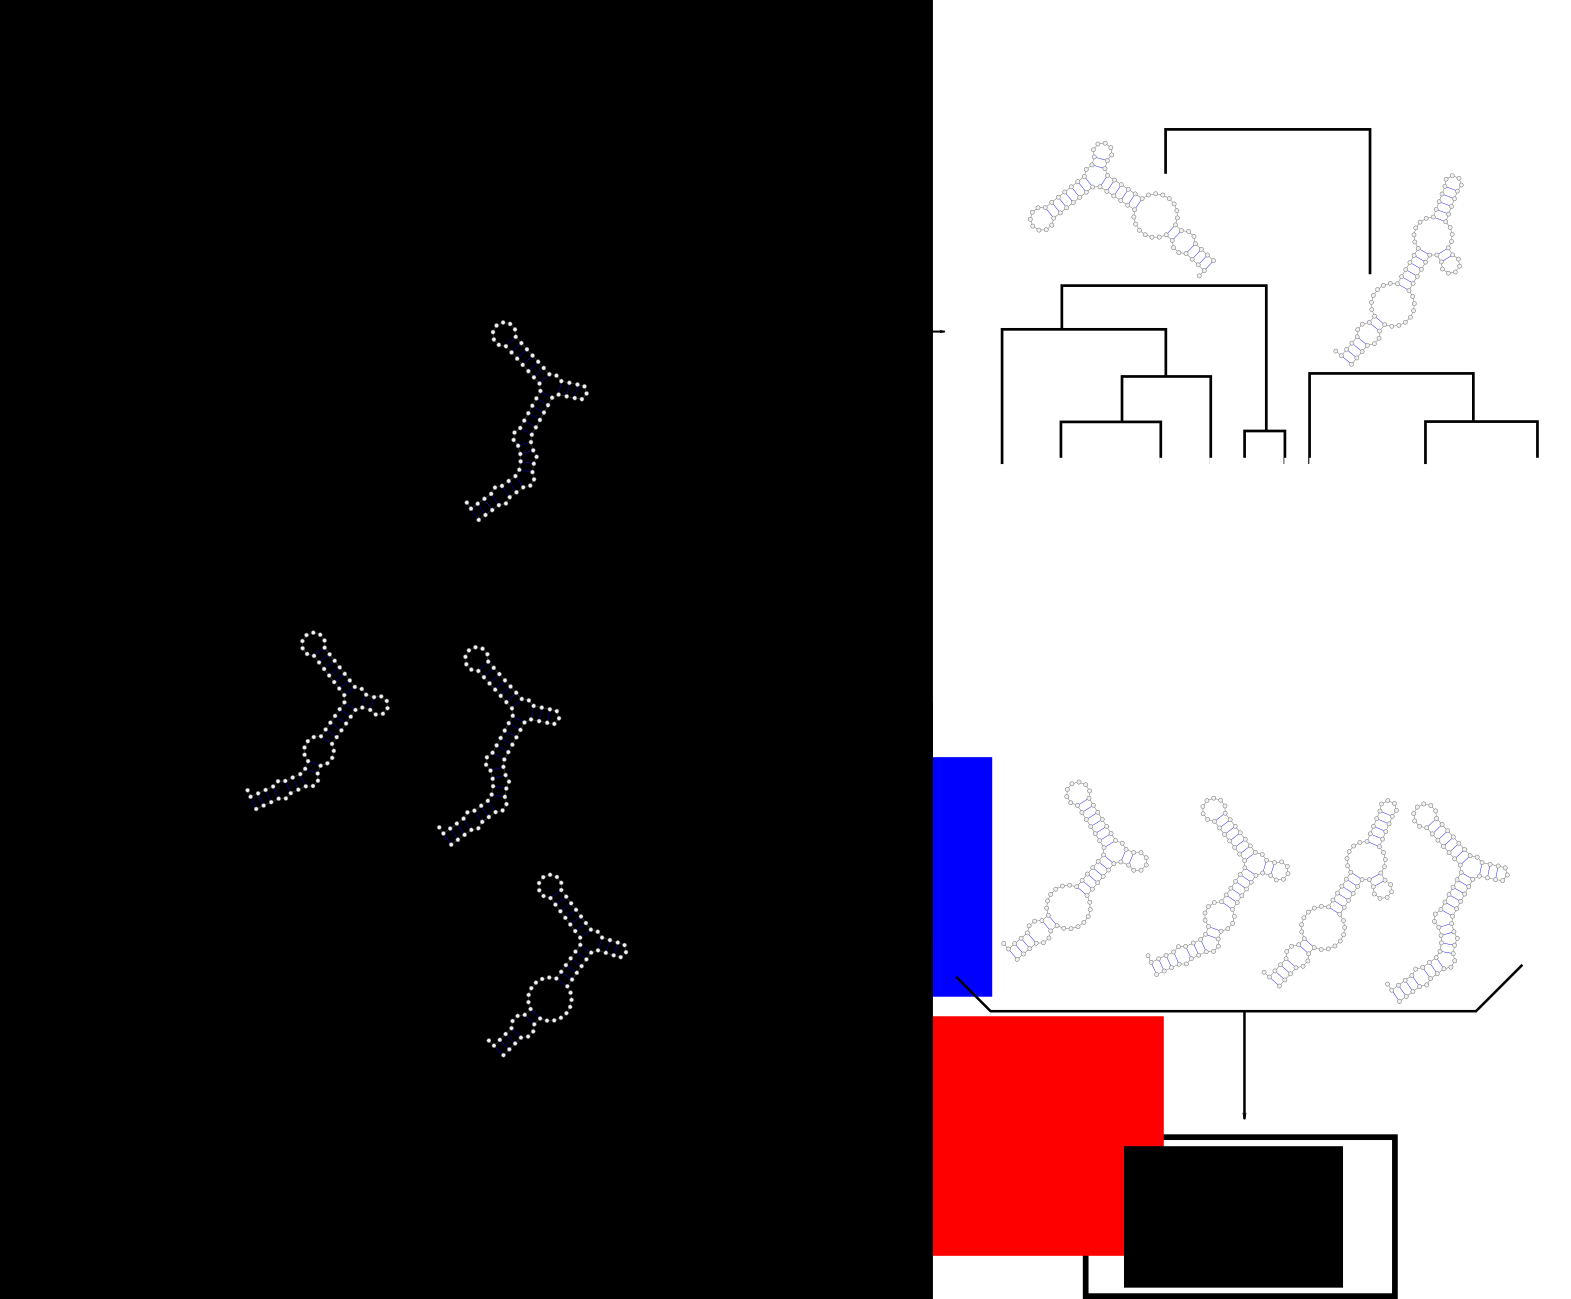
\includegraphics[width=0.9\textwidth]{/home/tsuname/Documents/lab/rhiju/papers/REEFFIT/structselect.png}
\caption{Selection algorithm for obtaining the structure set used to model the data when no structural ensemble is given \textit{a priori}. (A) An initial set of structures is calculated by clustering the suboptimal structures for all sequences in the experiment. Initial structure medoids are those that maximize a $score$ function that favors structures that are seen to be most stabilized in some measurement/mutant. (B) Additional structures from a sequence of $score$-sorted structures are added until the $AICc$ score, calculated within EM iterations, does not decrease further. The selected structures are finally re-fitted to the data using re-initialized variables in the REEFFIT statistical model model.}
\label{fig:structselectfig}
\end{figure}


\begin{figure}[here]
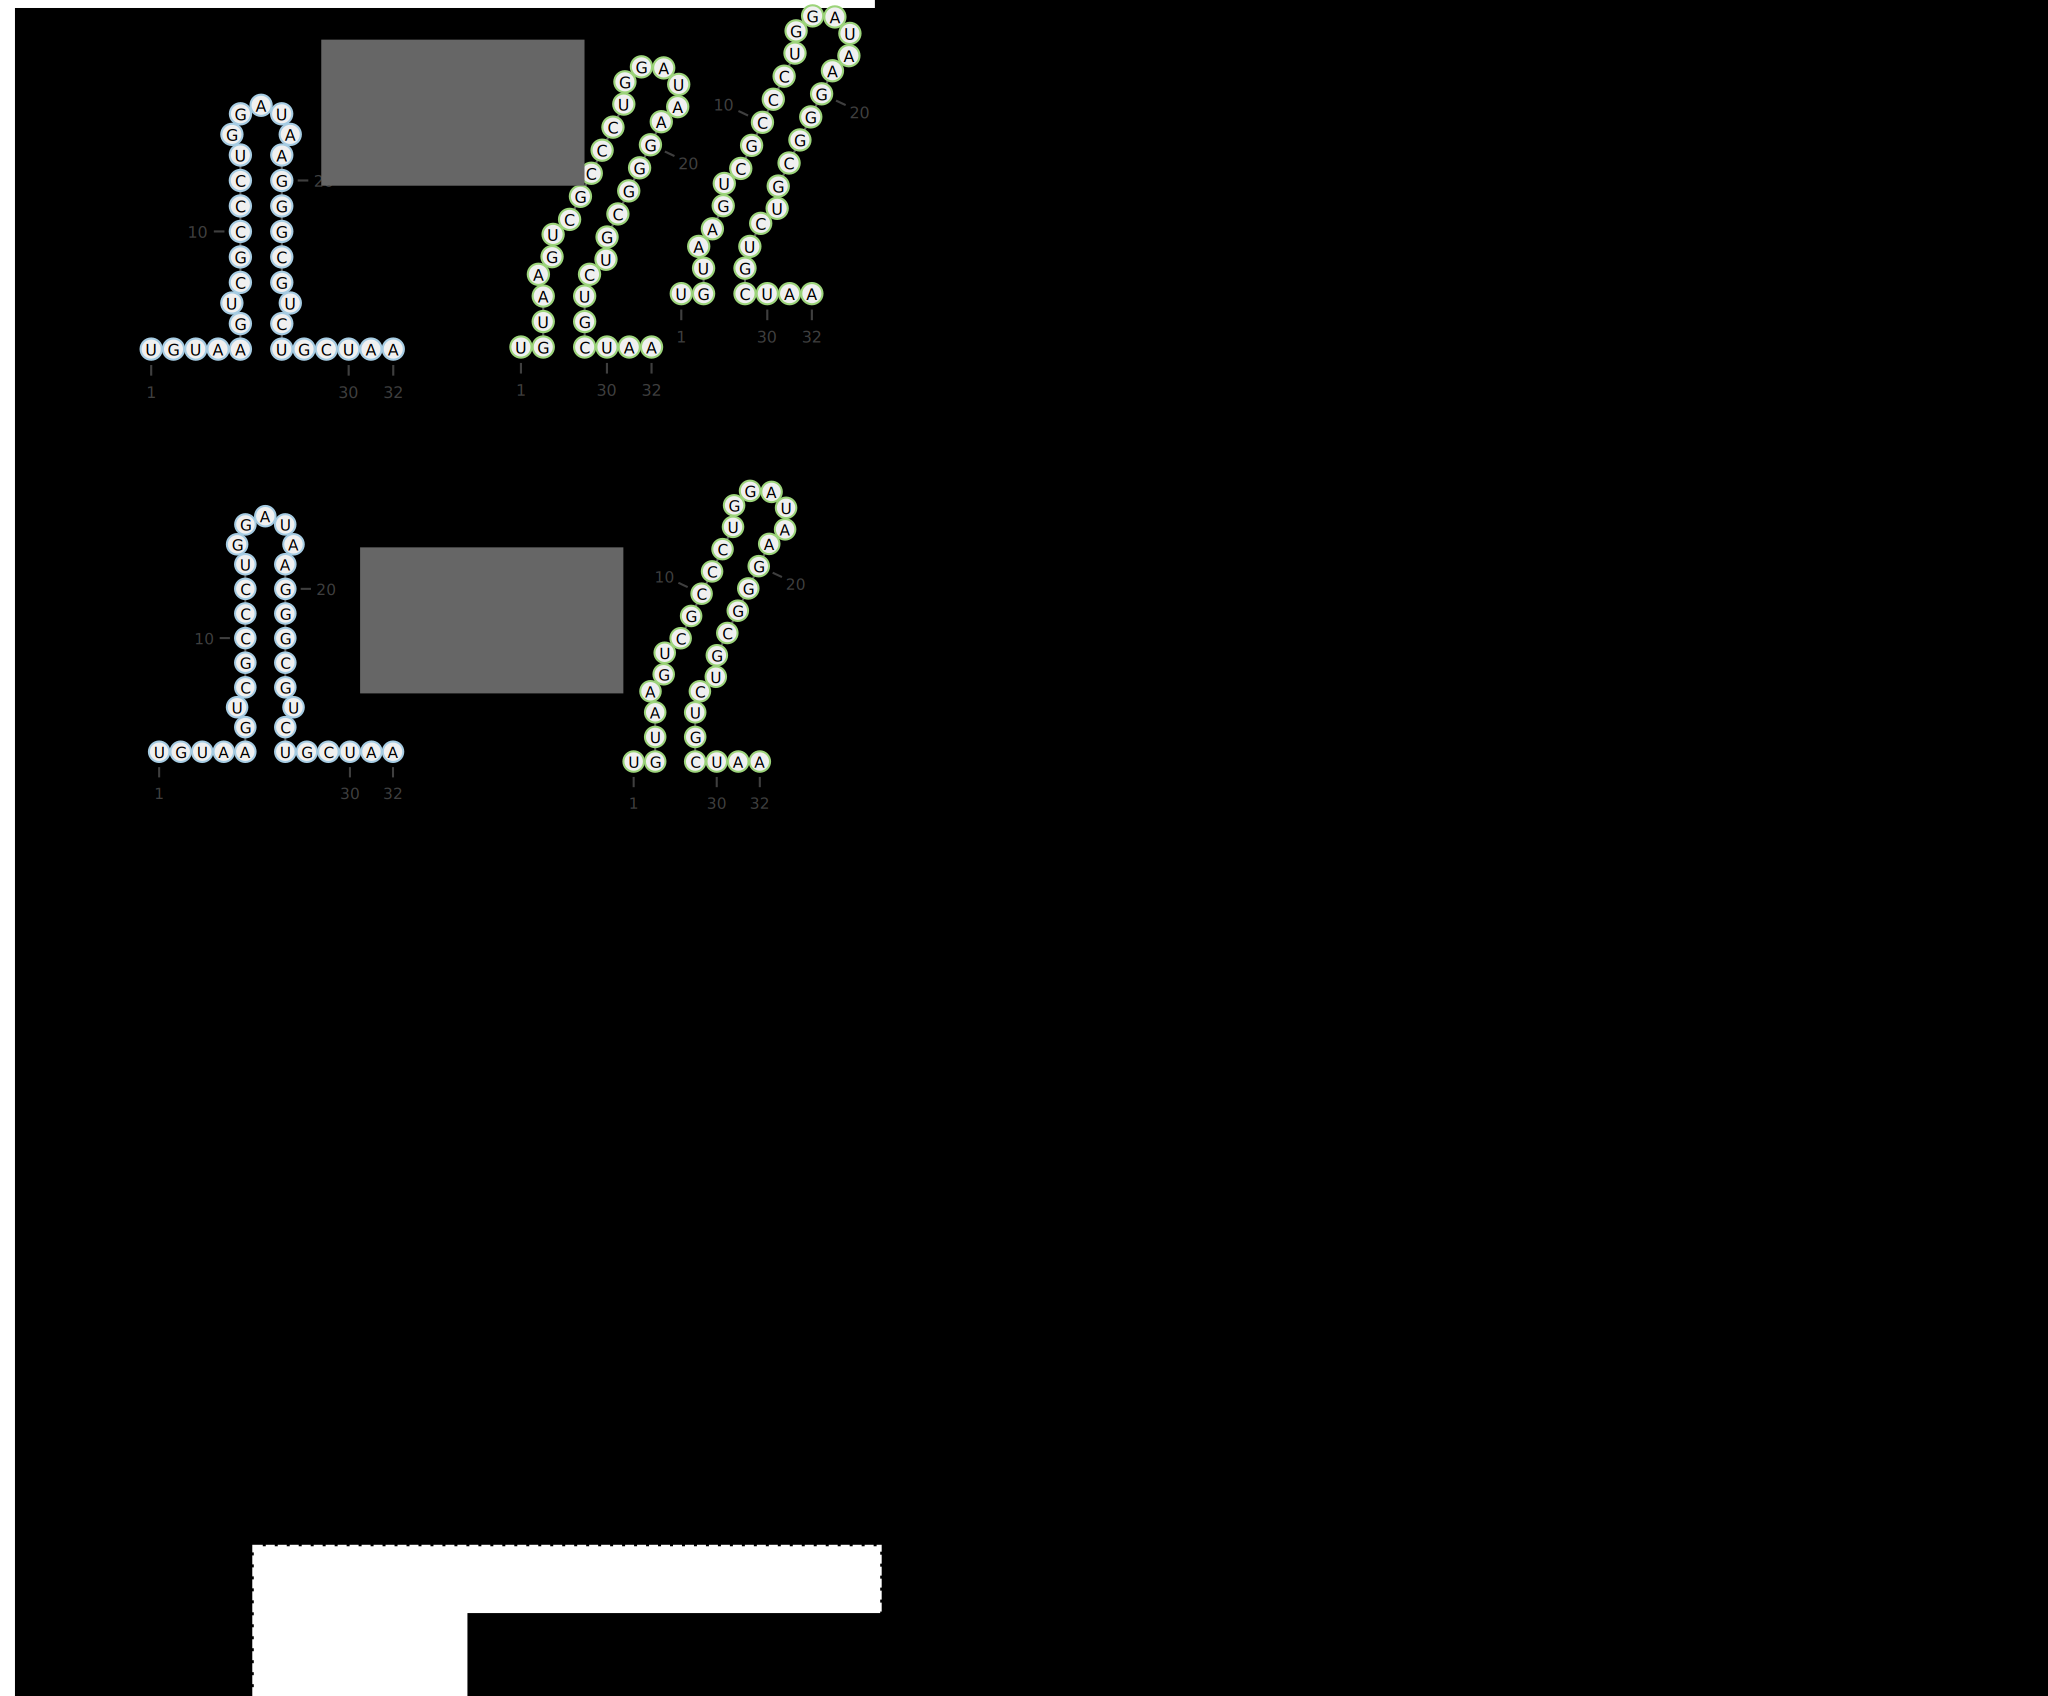
\includegraphics[width=0.9\textwidth]{/home/tsuname/Documents/lab/rhiju/papers/REEFFIT/rf00436_insilico.png}
\caption{Evaluation of the REEFIT method with simulated data. Here, we show the simulated data and REEFFIT analysis for an representative sequence of the RF00436 family. (A) Structures used for generating the data and those selected by REEFFIT to model the data. REEFFIT selected 2 structures, effectively collapsing two very similar generating structures into one structure (green). The other structure was identical to one of the structures used to generate the data (blue) (B) REEFFIT's predicted weights of each structure (solid lines with error bars, color-coded by structure color as in (A)) compared to the sums of true weights of structures per clusters defined by the two structure medoids (dotted lines, color-coded by structure medoid in each cluster as in (A)). Even though only two structures were used to model the data, the weights capture the underlying thermodynamic partition of the ensemble, assigning them correct weights. (C) Simulated M$^2$ data of the RF00436 representative, with noisy energies.  (D) Predicted data using REEFFIT's estimation for the structure weights, the expected values for the hidden chemical mapping profiles of each structure, and local mutation-induced perturbations. The predicted data is annotated with colored squares: red: observed data points that are not adequately captured by the model (less 0.05 probability of being generated by the estimated model); green/blue: positions where local perturbations induced by mutations are expected to occur in each structure, each square's transparency level is set proportional to the structure's weight at each mutant (the smaller the weight, the higher transparency value)}
\label{fig:insilicofig}
\end{figure}


%%%%%%%%%%HOBARTNER BIST FIGURES%%%%%%%%%%%%%%%%%%%%
\begin{figure}[here]
\includegraphics[width=0.9\textwidth]{/home/tsuname/Documents/lab/rhiju/papers/REEFFIT/hobartner.png}
\caption{M$^2$ measurements and predicted weights of the Hobartner bistable RNA structural ensemble. (A) The Hobartner bistable sequence folds into two different hairpins. (B) Weights calculated by REEFFIT for the wild type are within error from the NMR estimates (dotted horizontal lines).(C) M$^2$ measurements displayed in the same format as the simulated datasets in Figures ~\ref{fig:synthetichairpinfig} and ~\ref{fig:randomrnafig}. (D) Data predicted by the REEFFIT statistical model. Annotations are analogous to Figure ~\ref{fig:synthetichairpinfig}.}.
\label{fig:hobartnerfig}
\end{figure}

\begin{figure}[here]
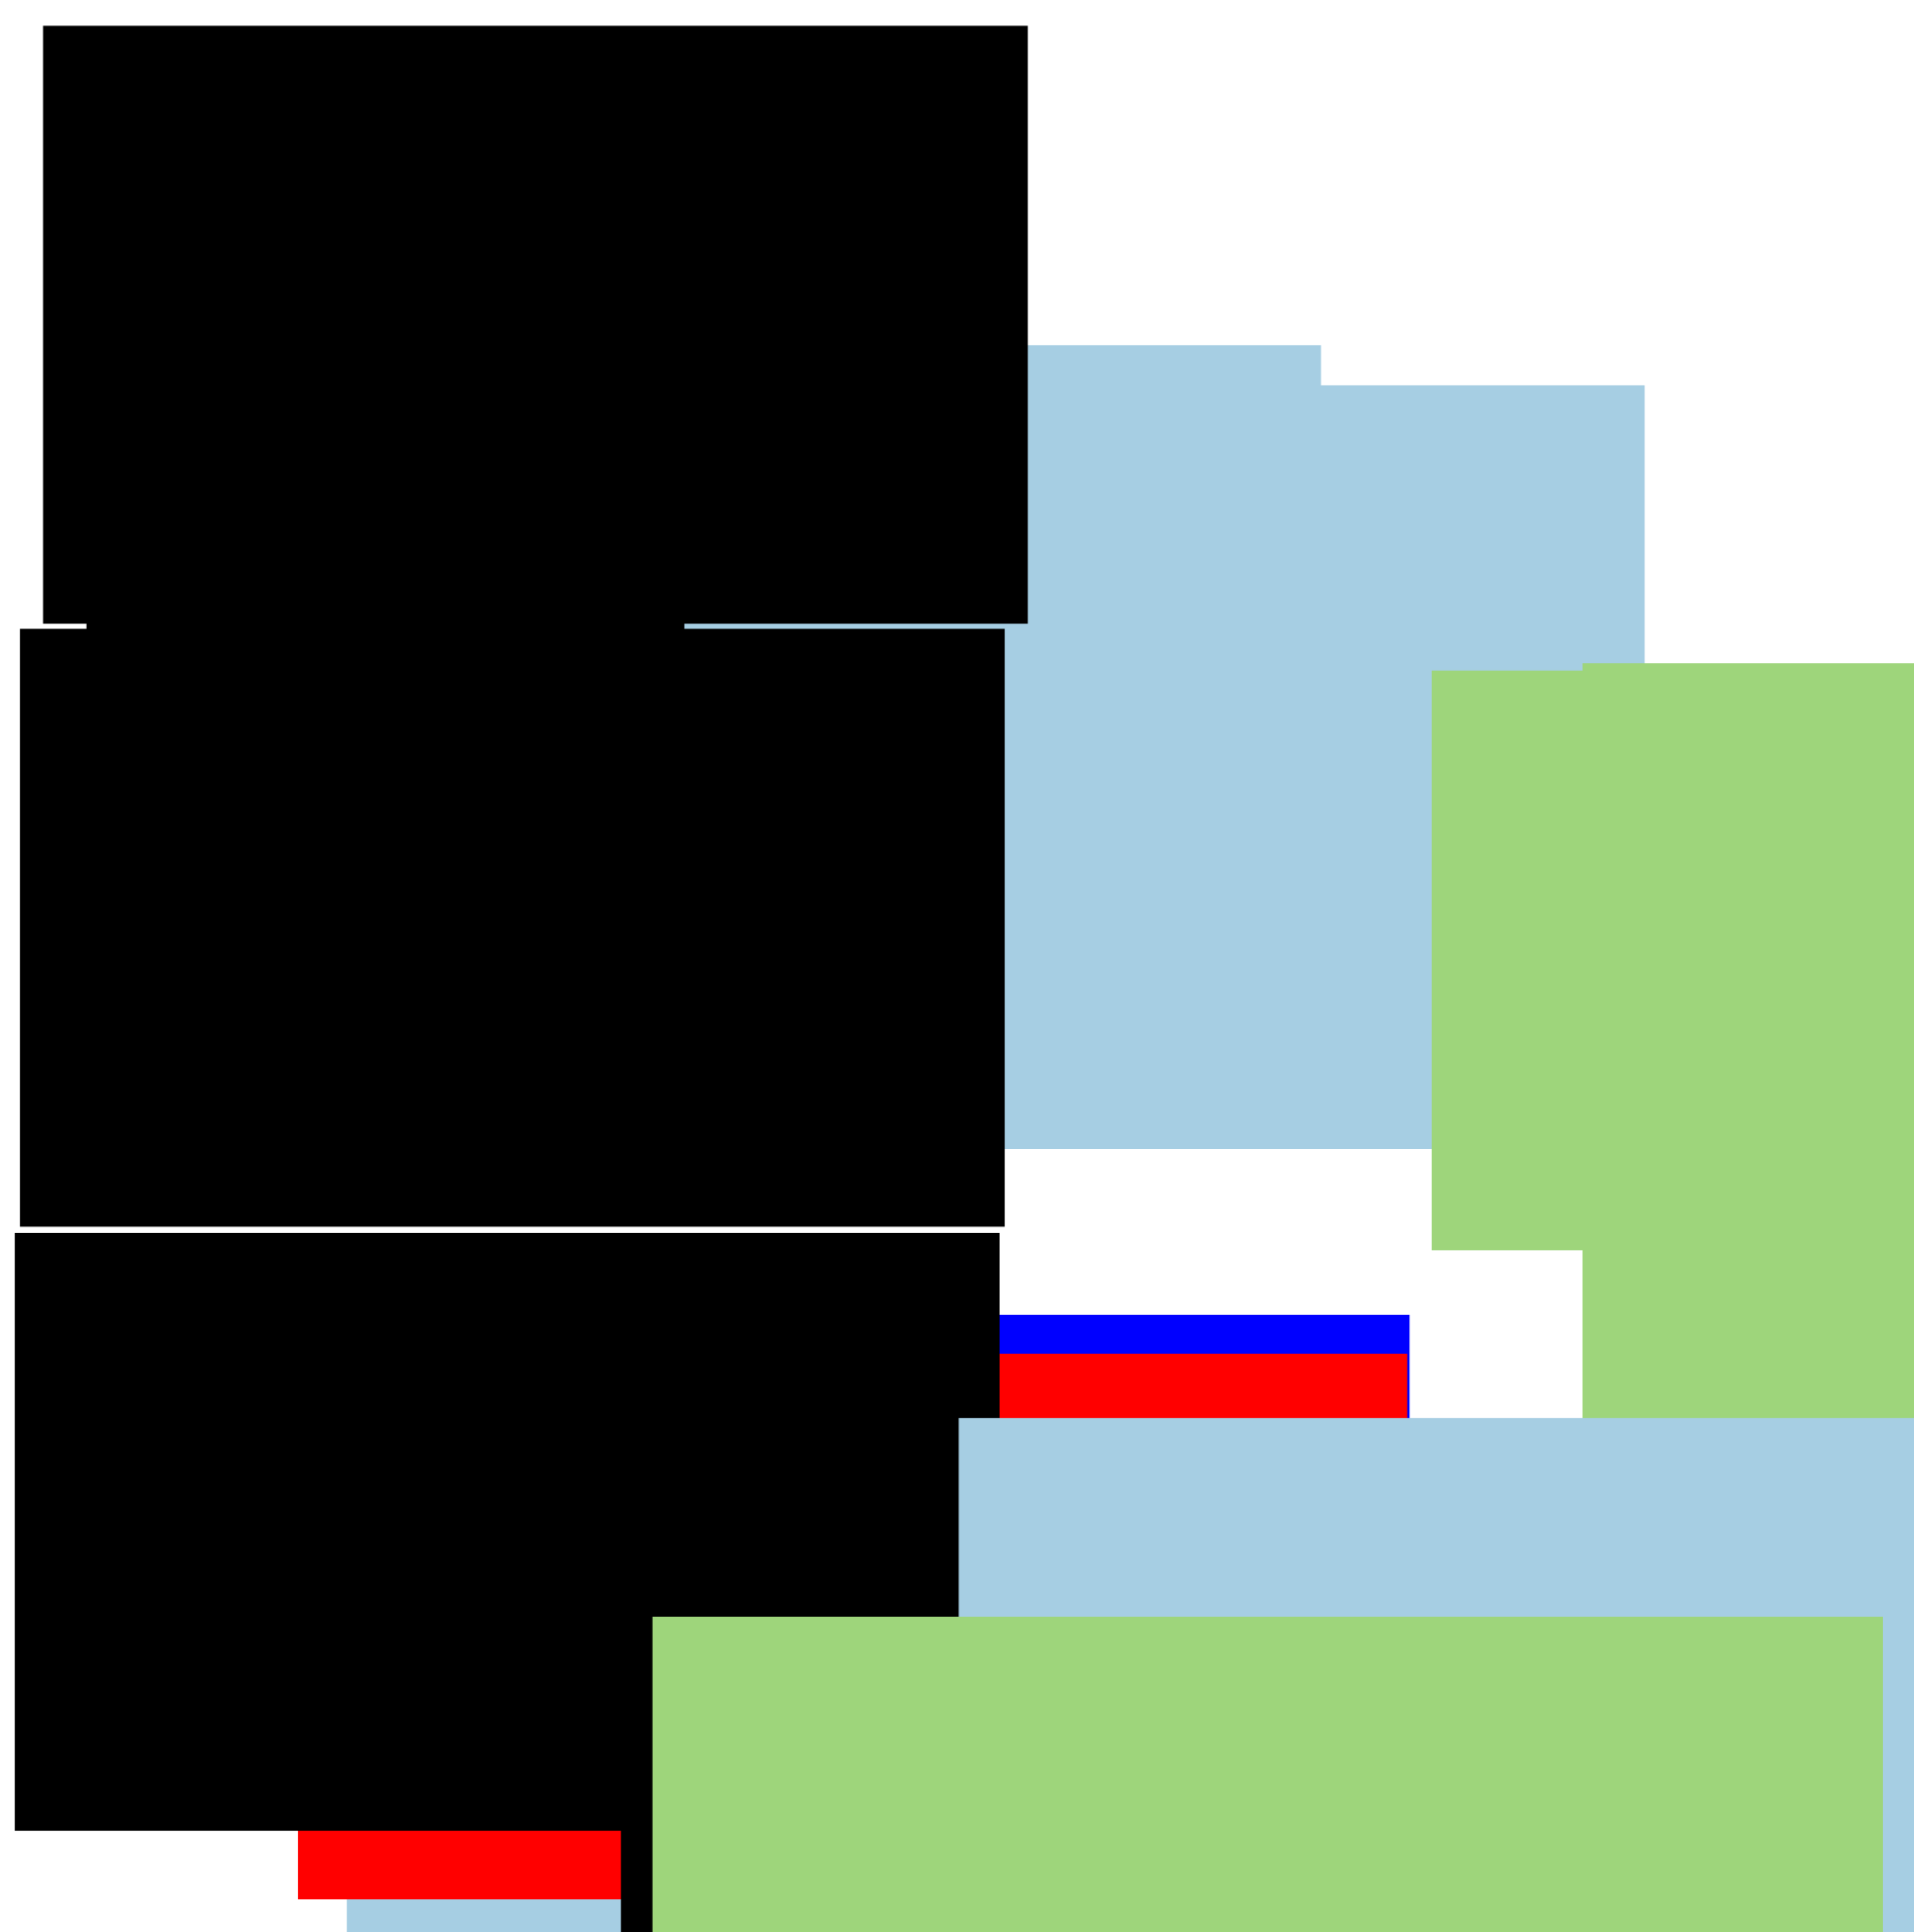
\includegraphics[width=0.9\textwidth]{/home/tsuname/Documents/lab/rhiju/papers/REEFFIT/hobartnervalidation.png}
\caption{Reactivities of the wild type Hobartner bistable RNA as a function of two mutants that are predicted by REEFFIT to fully stabilize each structure in the structural ensemble. (A) A4U is predicted to fold predominantly in structure $hob_1$ (blue); (B) C23G is most of the time in state $hob_2$ (green). (C) Combining their profiles with weights 0.7 for A4U and 0.3 for G23C (blue) results in reactivities similar to the wild type profile (red). The differences between the weighted combination of mutants and the wild type reactivities can be explained by their respective mutations and their effects on their helix partners in each state (blue and green stars, for mutants A4U and C23G, respectively).}.
\label{fig:hobartnervalidationfig}
\end{figure}



%%%%%%%%%%MEDLOOP FIGURES%%%%%%%%%%%%%%%%%%%%

\begin{figure}[here]
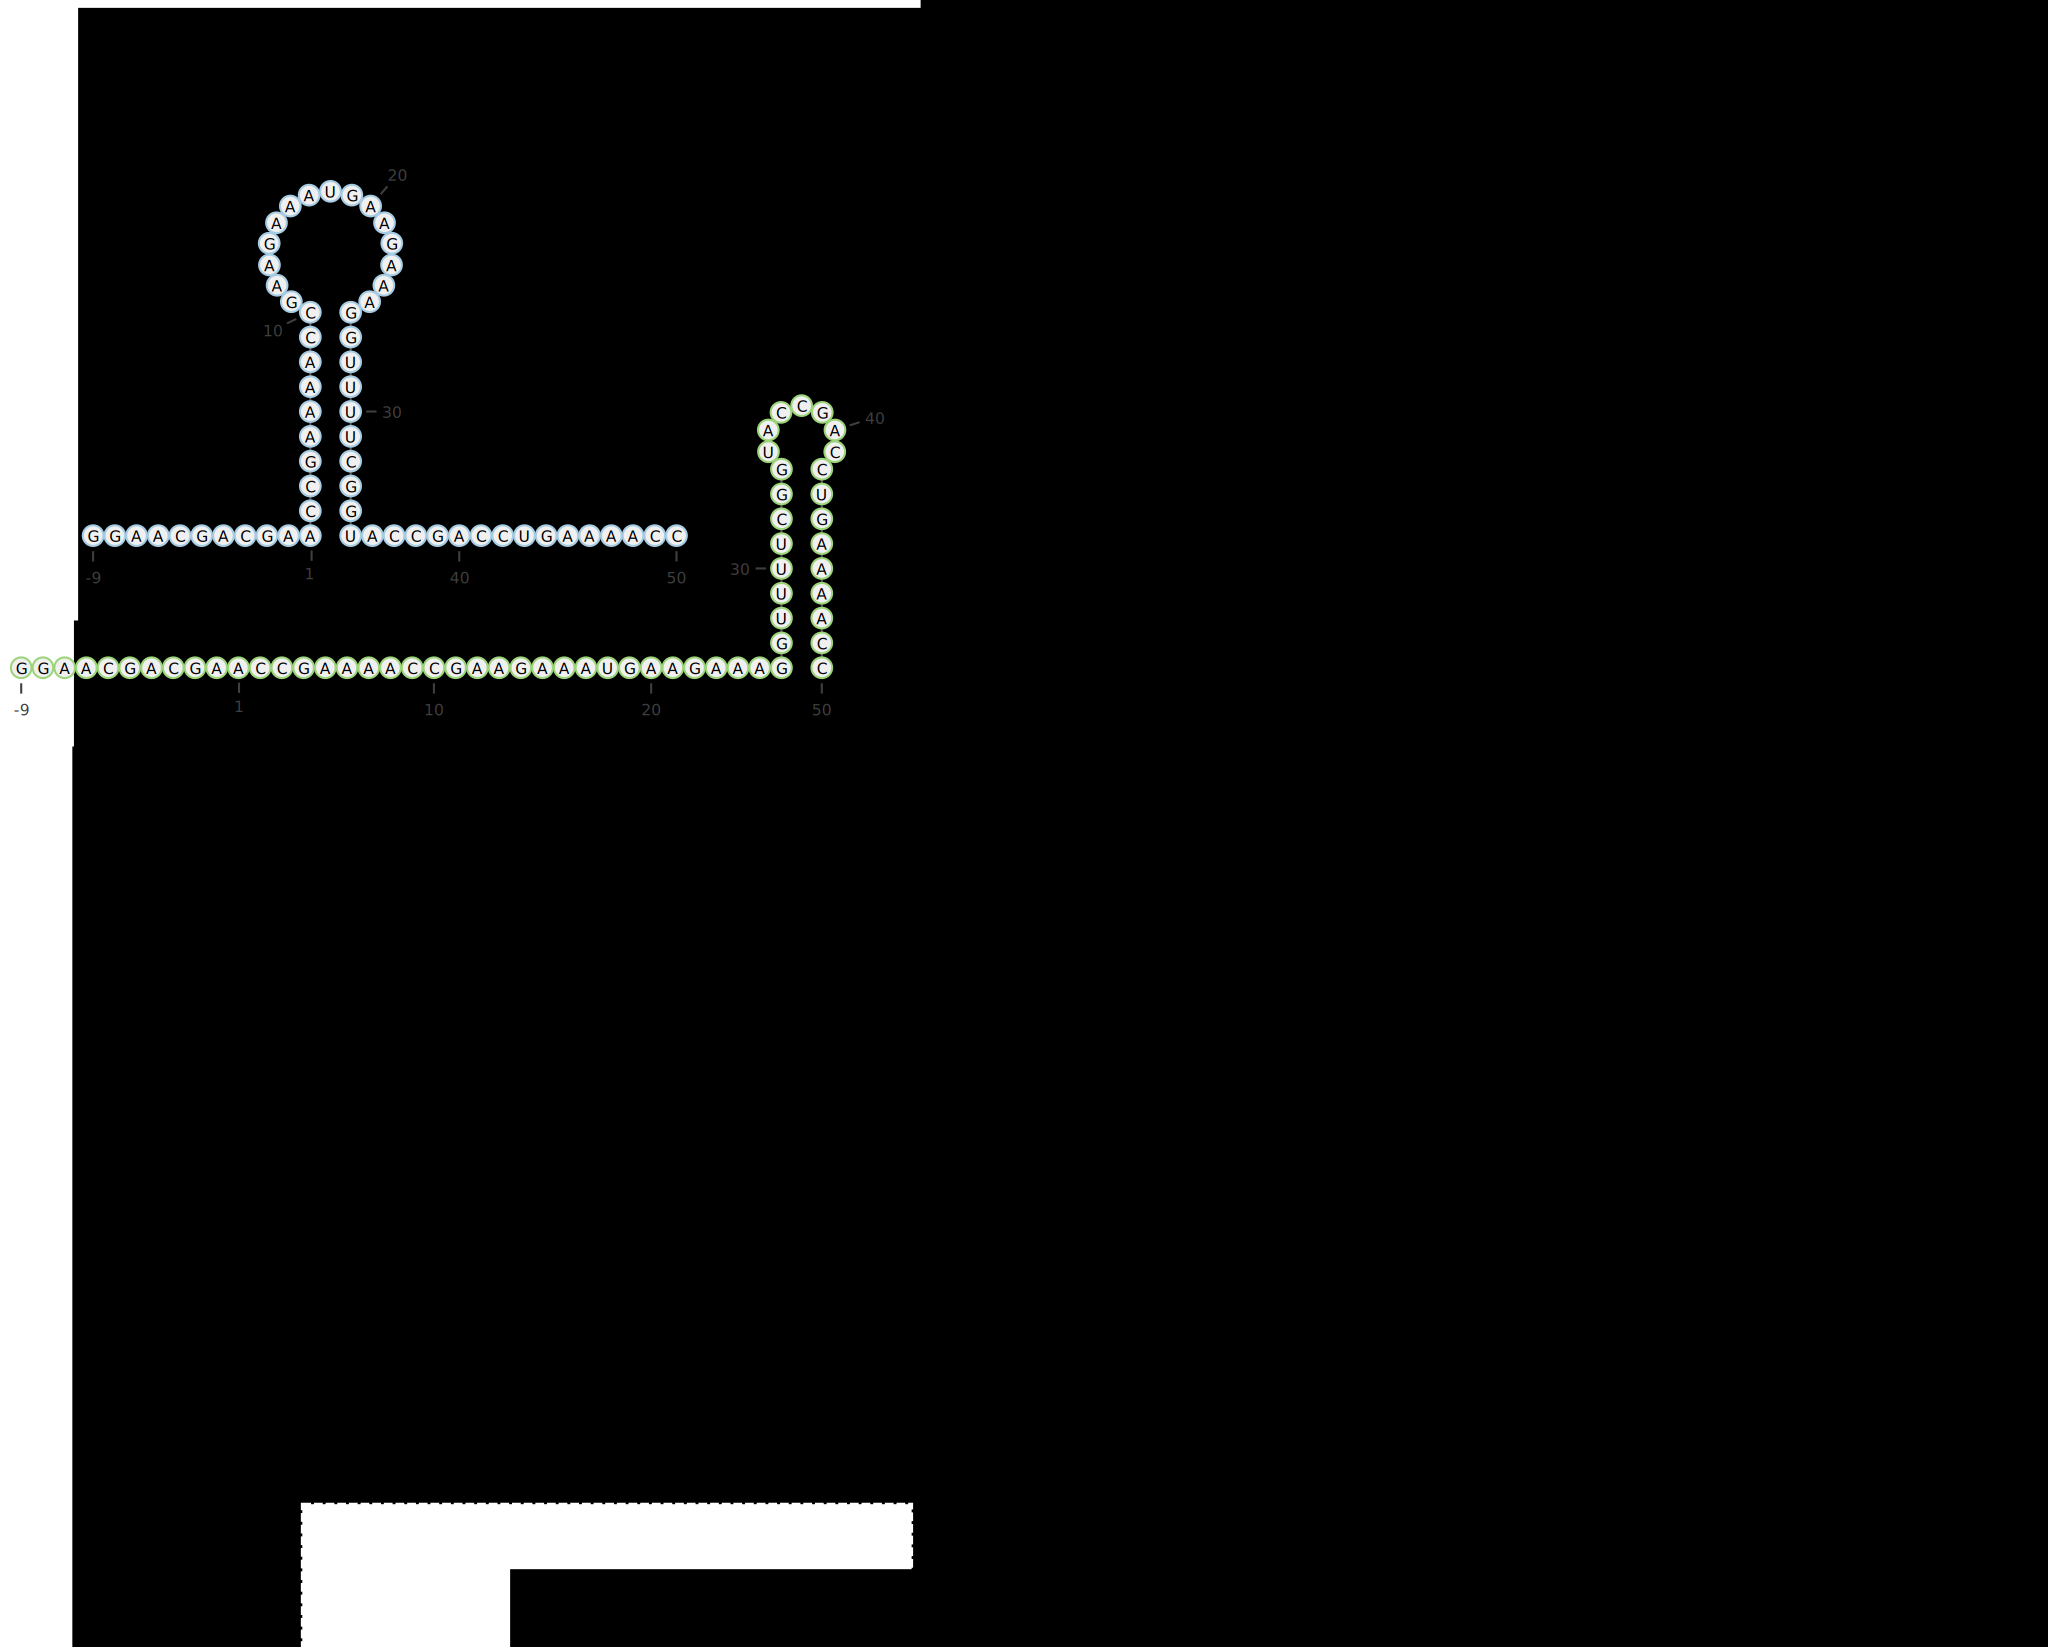
\includegraphics[width=0.9\textwidth]{/home/tsuname/Documents/lab/rhiju/papers/REEFFIT/medloop.png}
\caption{M$^2$-seq measurements and predicted weights of the MedLoop motif. (A) Structures selected by REEFFIT to model the data. One structure (blue) is predominant in most mutants; mutations that severly disrupt it (e.g. G4C) form an alternative structure (green)  (B) M$^2$ measurements displayed in the same format as the simulated datasets in Figures ~\ref{fig:synthetichairpinfig} and ~\ref{fig:randomrnafig}. (C) Data predicted by the REEFFIT statistical model. Annotations are analogous to Figure ~\ref{fig:synthetichairpinfig}. (D) Comparison of observed reactivities for the wild type MedLoop sequence to the predicted profile of REEFFIT.}.
\label{fig:medloopfig}
\end{figure}

%%%%%%%%%%MEDLOOP DELTA FIGURES%%%%%%%%%%%%%%%%%%%%
\begin{figure}[here]
\includegraphics[width=0.7\textwidth]{/home/tsuname/Documents/lab/rhiju/papers/REEFFIT/medloopdelta.png}
\caption{M$^2$-seq measurements and predicted weights of the MedLoop$\Delta$ construct. (A) Structures selected by REEFFIT to model the data. MedLoop$\Delta$ shares one structure with the MedLoop RNA (blue), but lacks the nucleotides for the alternative structure. Because of this deletion, another two alternative structures are stabilized by some of the mutants (green and red) (B) M$^2$ measurements displayed in the same format as the simulated datasets in Figures ~\ref{fig:synthetichairpinfig} and ~\ref{fig:randomrnafig}. (C) Data predicted by the REEFFIT statistical model. Annotations are analogous to Figure ~\ref{fig:synthetichairpinfig}.}.
\label{fig:medloopdeltafig}
\end{figure}


%%%%%%%%%%M-STABLE FIGURES%%%%%%%%%%%%%%%%%%%%
\begin{figure}[here]
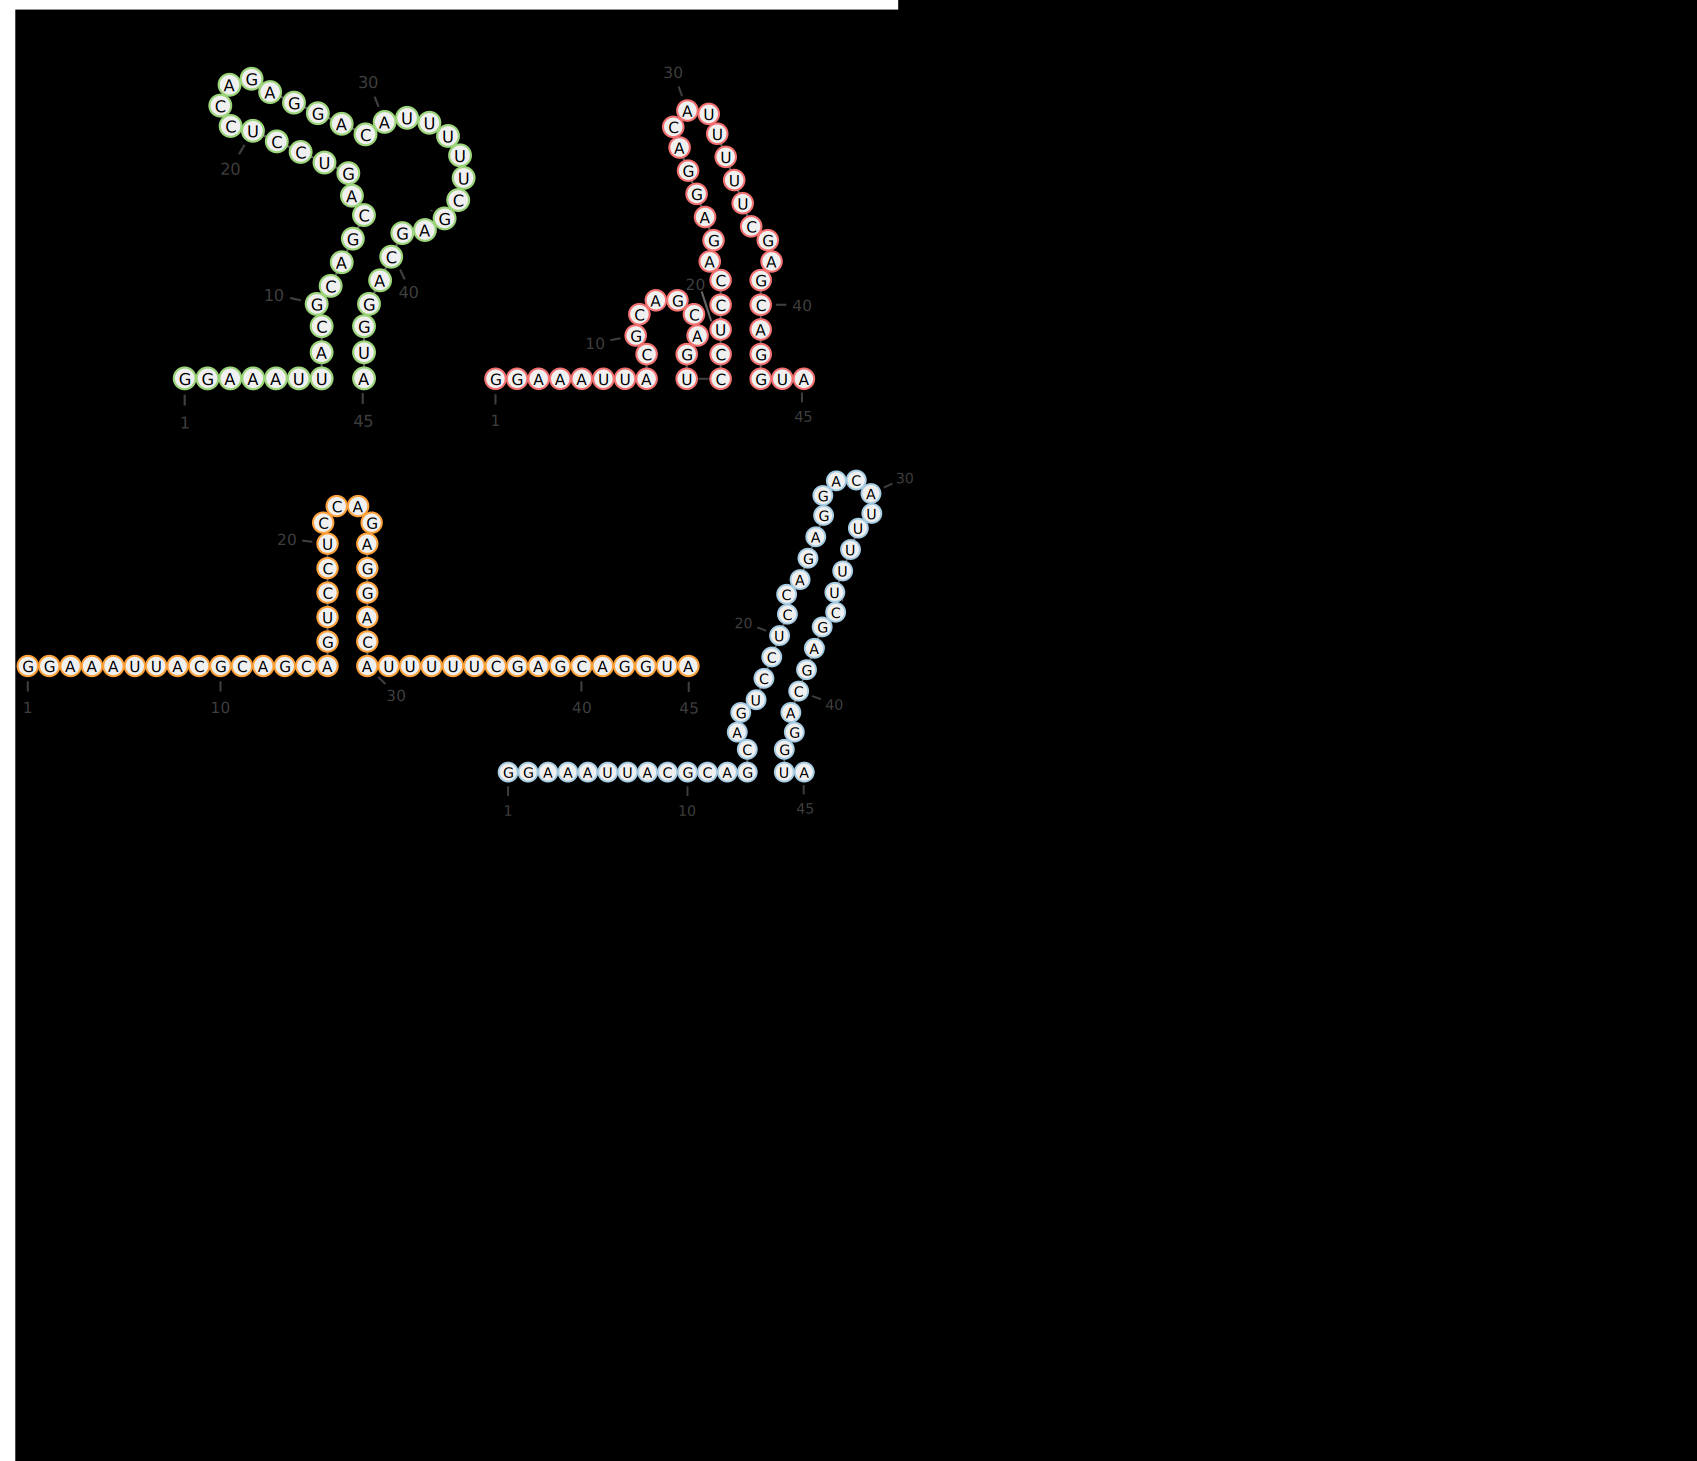
\includegraphics[width=0.9\textwidth]{/home/tsuname/Documents/lab/rhiju/papers/REEFFIT/mstable.png}
\caption{M$^2$-seq measurements and predicted weights of the M-stable RNA. (A) Structures selected by REEFFIT to model the data. MedLoop$\Delta$ shares one structure with the MedLoop RNA (blue), but lacks the nucleotides for the alternative structure. Because of this deletion, another two alternative structures are stabilized by some of the mutants (green and red) (B) M$^2$ measurements displayed in the same format as the simulated datasets in Figures ~\ref{fig:synthetichairpinfig} and ~\ref{fig:randomrnafig}. (C) Data predicted by the REEFFIT statistical model. Annotations are analogous to Figure ~\ref{fig:synthetichairpinfig}.}.
\label{fig:mstablefig}
\end{figure}


%%%%%%%%%%%%%% Supplemental Figures %%%%%%%%%%%%%%
%%%%%%%%%%HOBARTNER BIST FIGURES%%%%%%%%%%%%%%%%%%%%

\begin{figure}[here]
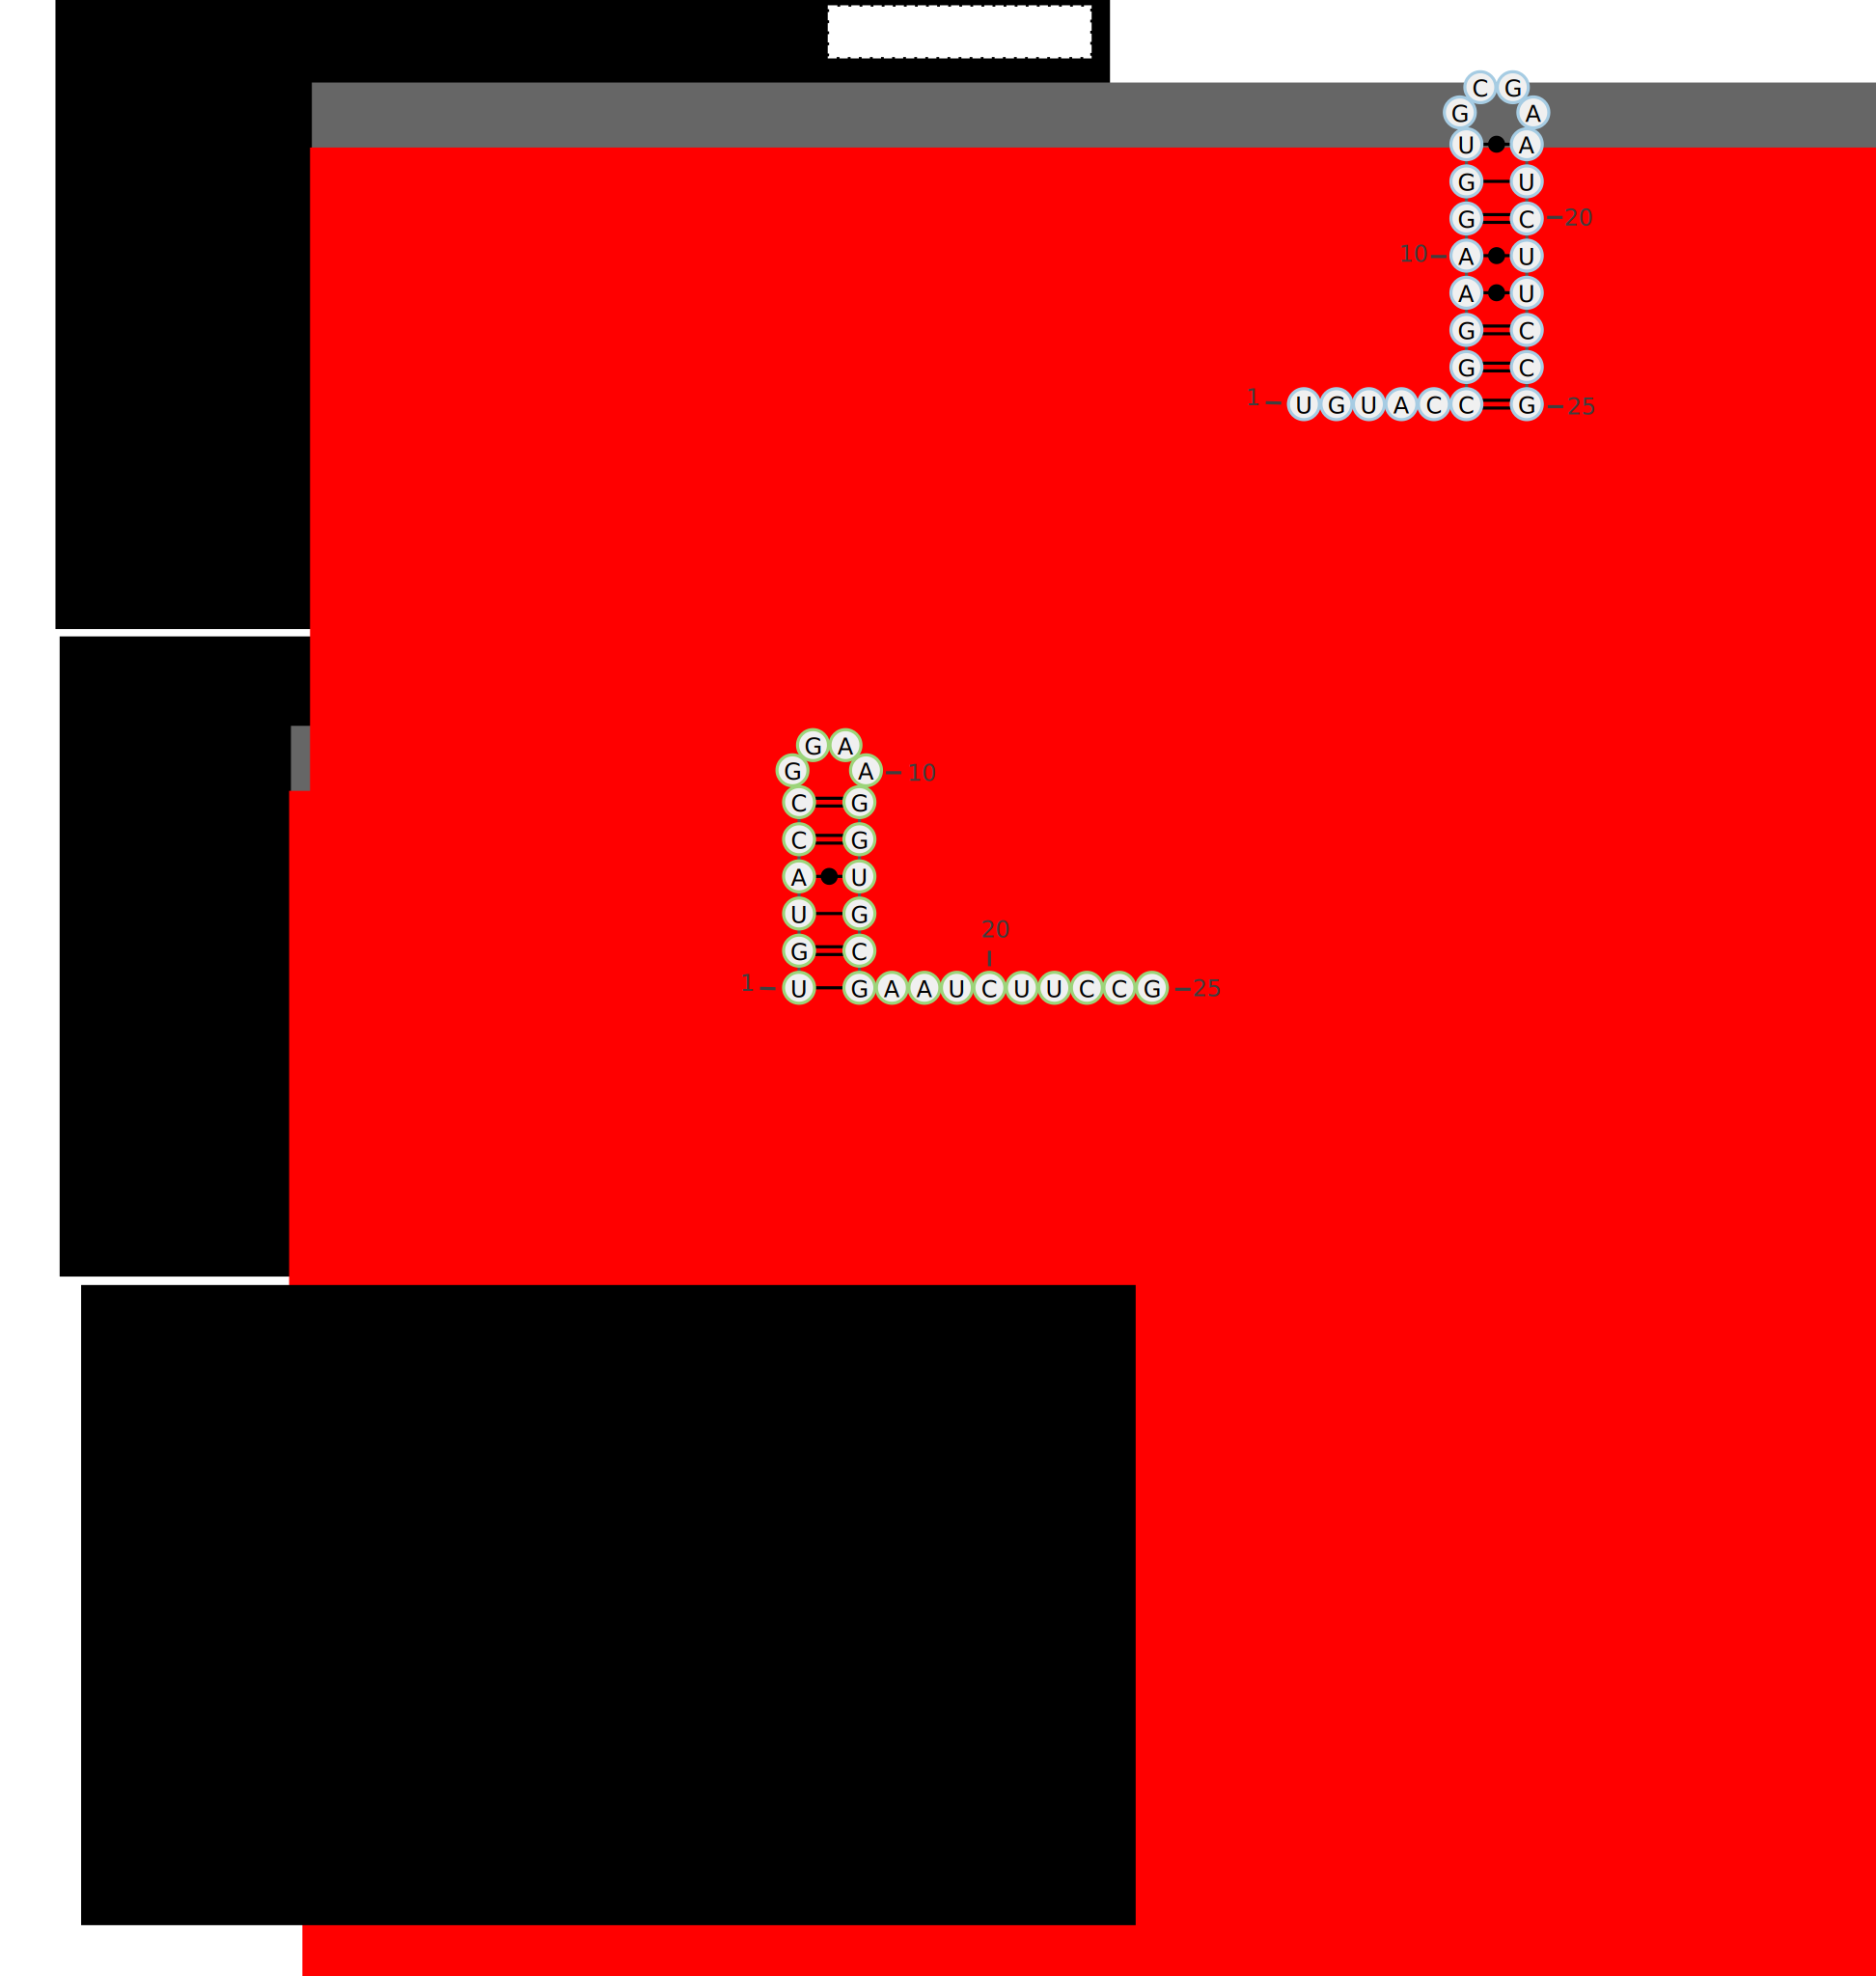
\includegraphics[width=0.9\textwidth]{/home/tsuname/Documents/lab/rhiju/papers/REEFFIT/hobartnerpredicted.png}
\caption{Expected and predicted reactivities for the two structures in the Hobartner bistable RNA ensemble. (A,B) Expected reactivities of the calculated by MCMC simulations. The solid red lines indicates our prior for each sequence position in each sructure (zero or one, for paired and unpaired residues in that structure, respectively)(C)  Comparison of observed reactivities for the wild type Hobartner sequence to the predicted profile of REEFFIT. Error bars are the estimated value for $\Psi_i$ at each position.}.
\label{fig:hobartnerpredictedfig}
\end{figure}


%%%%%%%%%%MEDLOOP FIGURES%%%%%%%%%%%%%%%%%%%%
\begin{figure}[here]
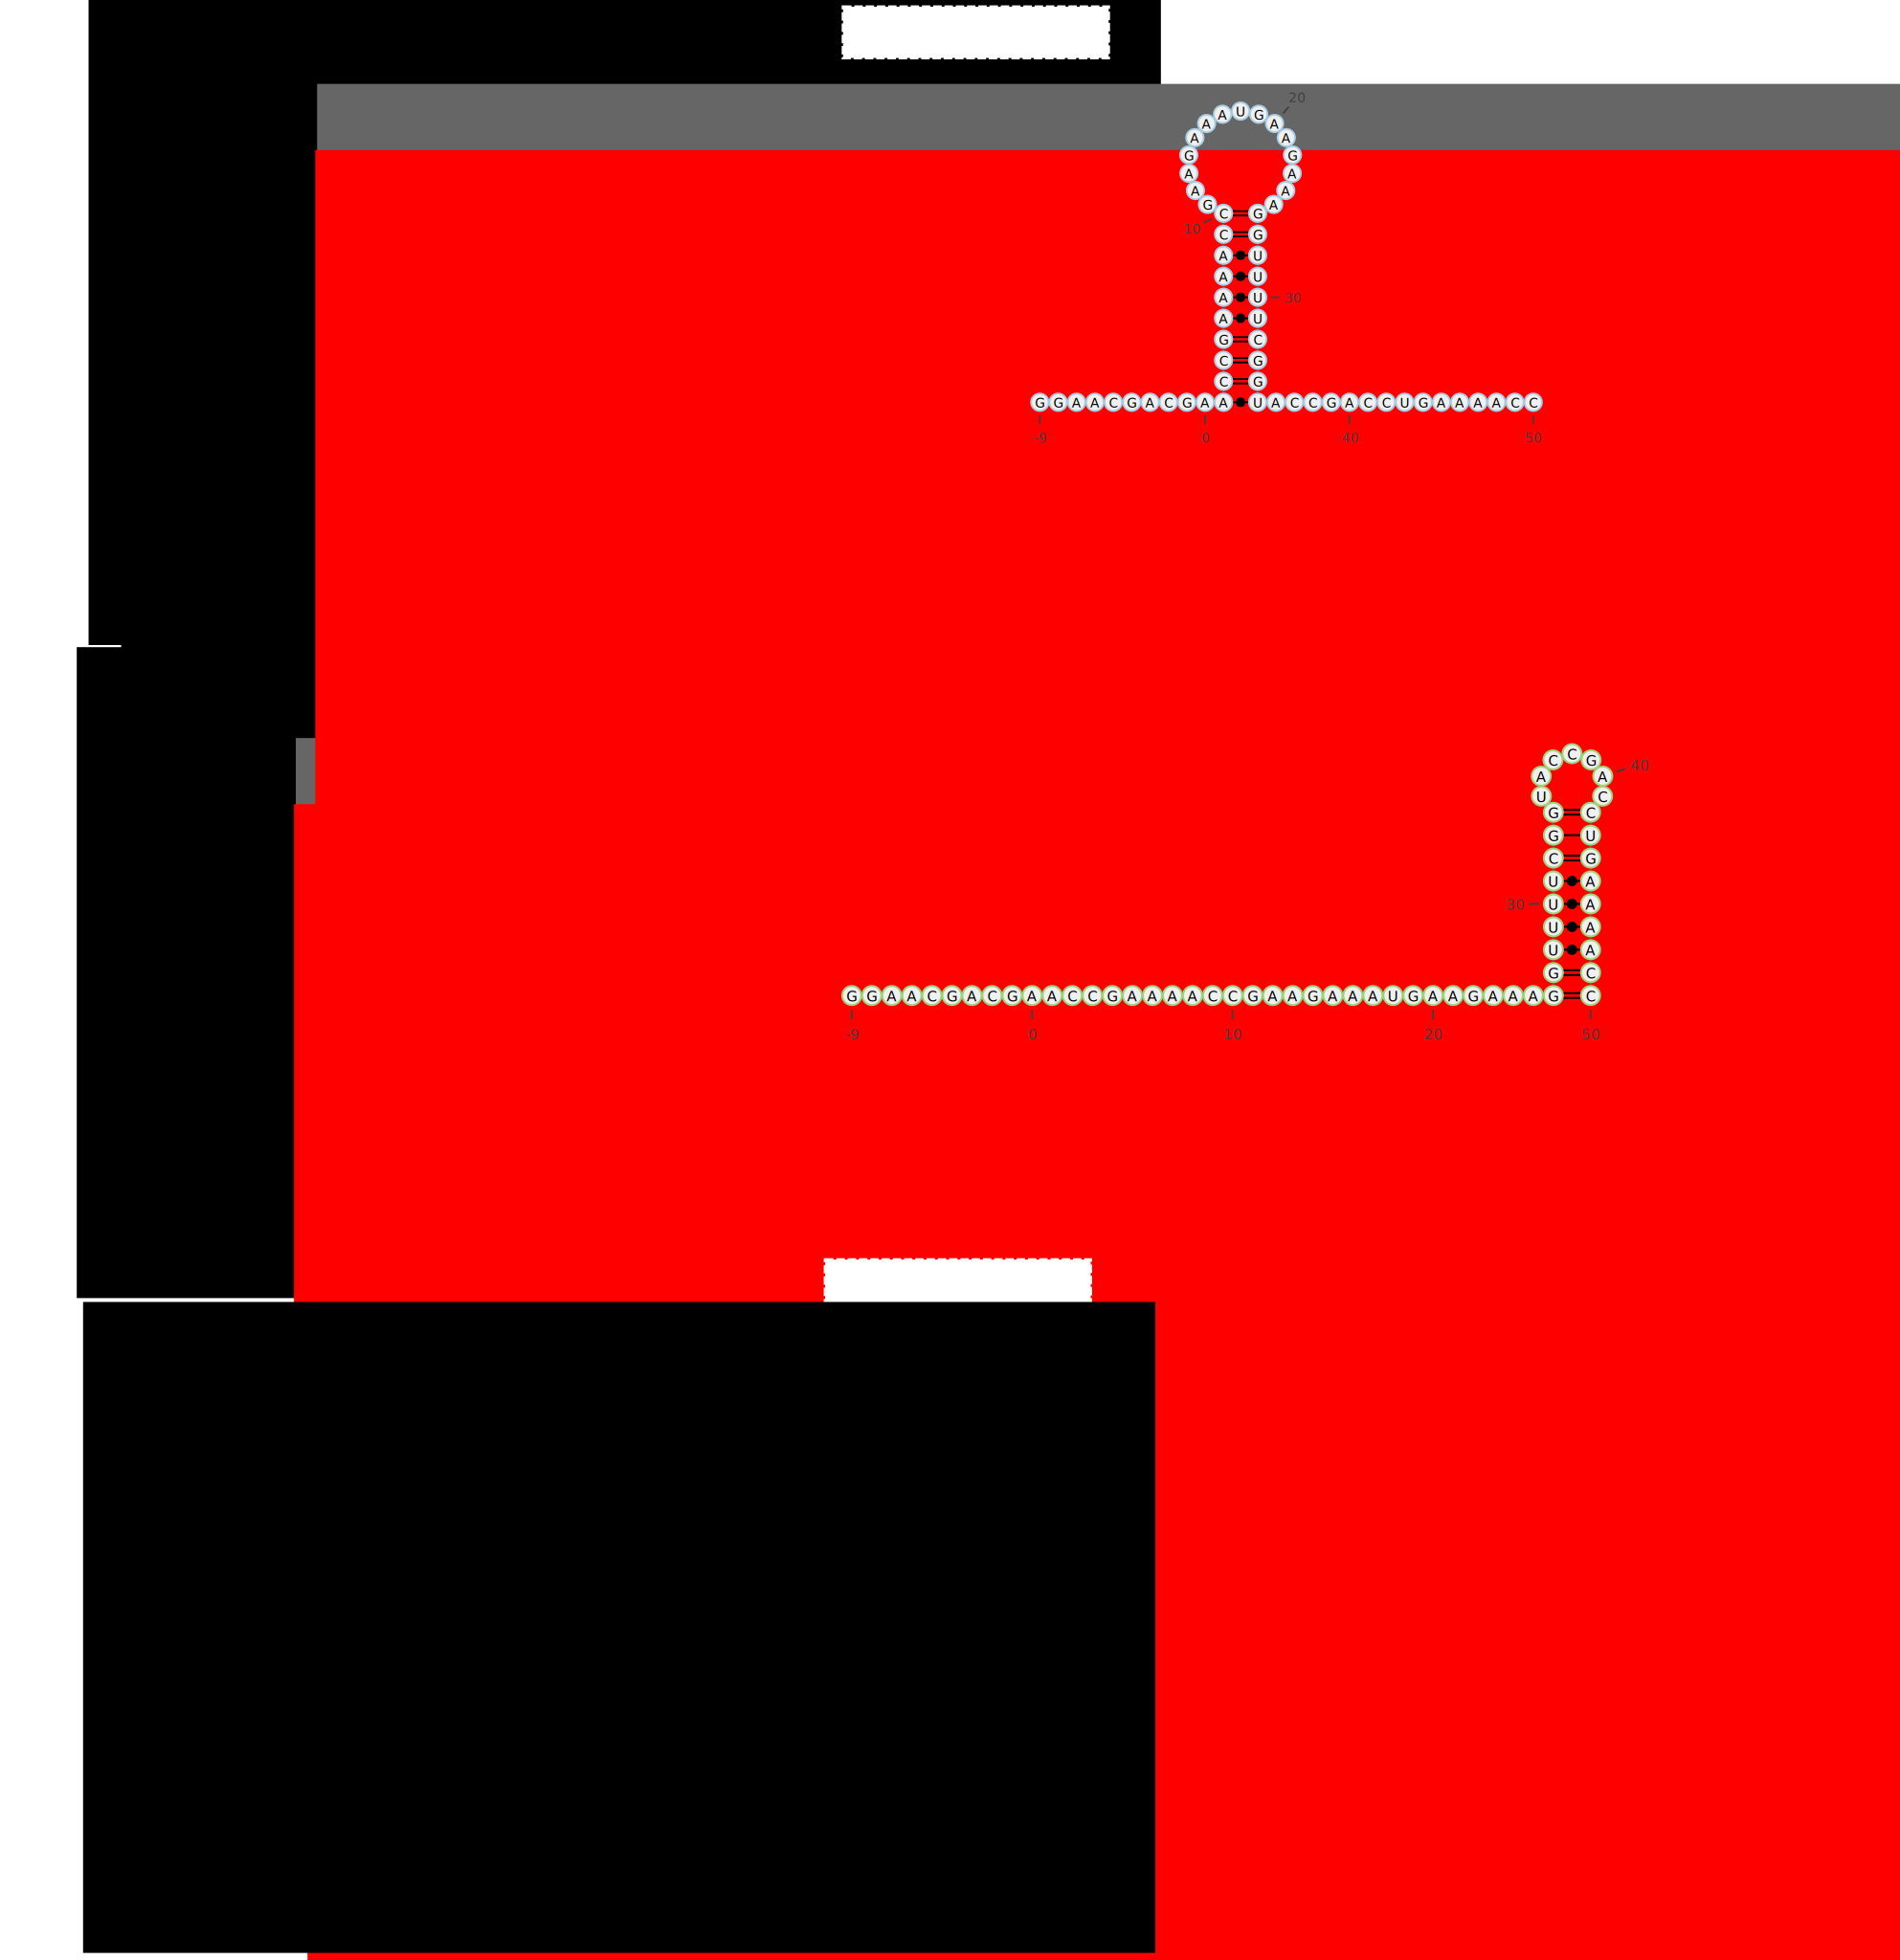
\includegraphics[width=0.9\textwidth]{/home/tsuname/Documents/lab/rhiju/papers/REEFFIT/medlooppredicted.png}
\caption{Expected and predicted reactivities for the two structures in the MedLoop RNA ensemble. (A,B) Expected reactivities of the two structures calculated by MCMC simulations. The solid red lines indicates our prior for each sequence position in each sructure (zero or one, for paired and unpaired residues in that structure, respectively)(C)  Comparison of observed reactivities for the wild type MedLoop sequence to the predicted profile of REEFFIT. Error bars are the estimated value for $\Psi_i$ at each position.}.
\label{fig:medlooppredictedfig}
\end{figure}

%%%%%%%%%%MEDLOOP DELTA FIGURES%%%%%%%%%%%%%%%%%%%%

\begin{figure}[here]
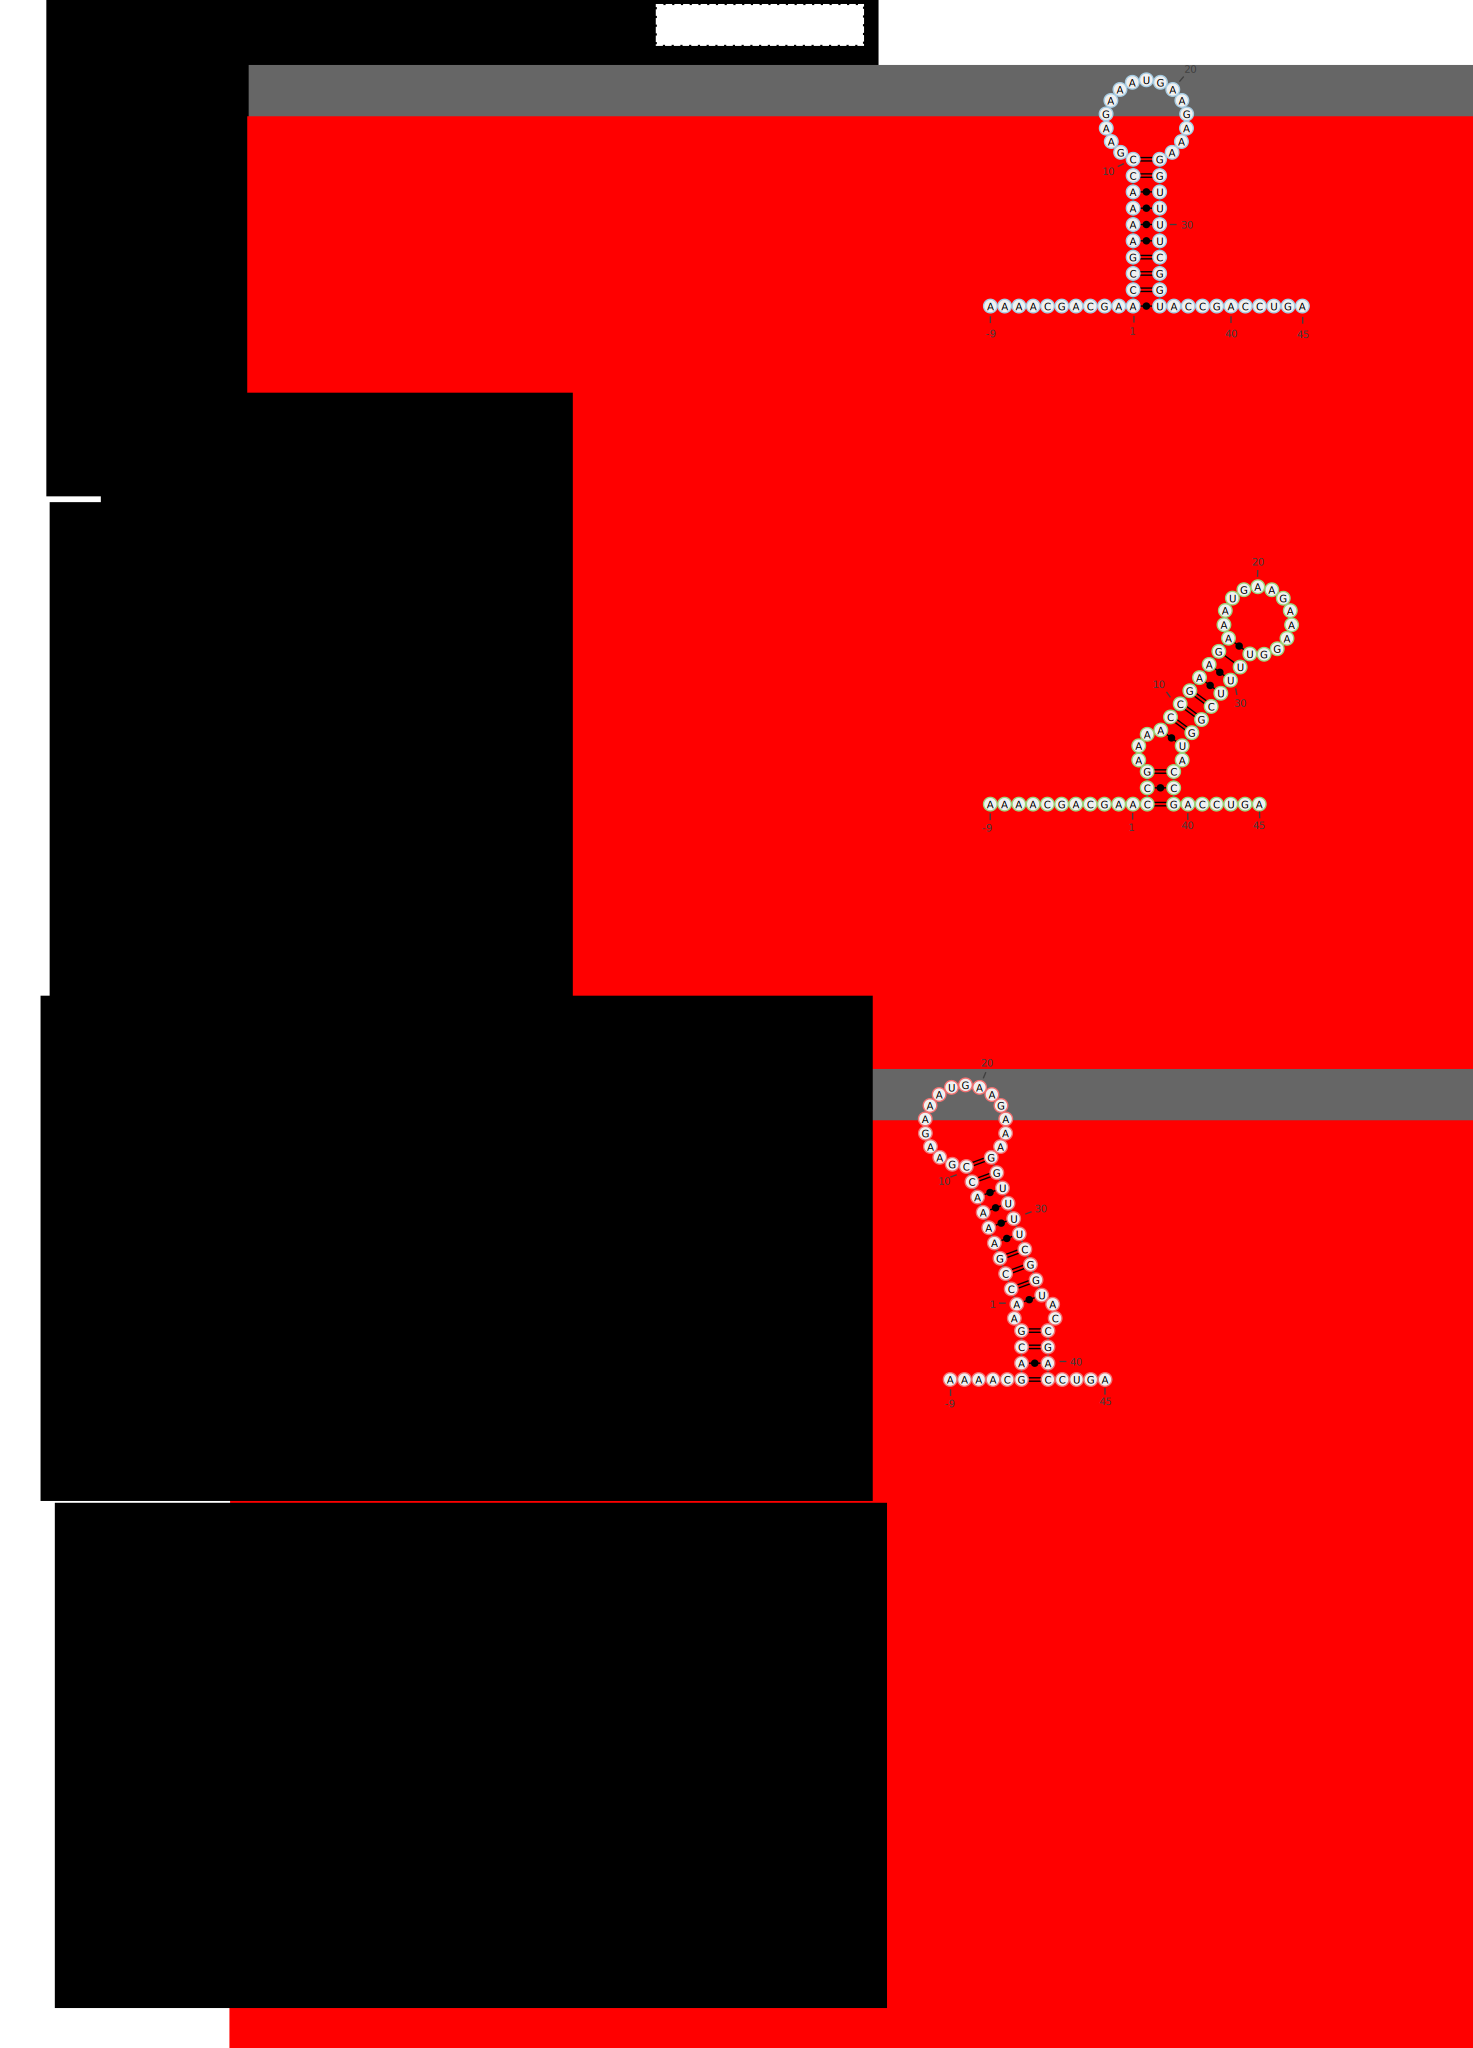
\includegraphics[width=0.9\textwidth]{/home/tsuname/Documents/lab/rhiju/papers/REEFFIT/medloopdeltapredicted.png}
\caption{Expected and predicted reactivities for the three structures in the MedLoop$\Delta$ RNA ensemble. (A-C) Expected reactivities of the three structures calculated by MCMC simulations. The solid red lines indicates our prior for each sequence position in each sructure (zero or one, for paired and unpaired residues in that structure, respectively)(D)  Comparison of observed reactivities for the wild type MedLoop$\Delta$ sequence to the predicted profile of REEFFIT. Error bars are the estimated value for $\Psi_i$ at each position.}.
\label{fig:medloopdeltapredictedfig}
\end{figure}

%%%%%%%%%%M-STABLE FIGURES%%%%%%%%%%%%%%%%%%%%
\begin{figure}[here]
\includegraphics[width=0.6\textwidth]{/home/tsuname/Documents/lab/rhiju/papers/REEFFIT/mstablepredicted.png}
\caption{Expected and predicted reactivities for the three structures in the M-stable RNA ensemble. (A-D) Expected reactivities of the three structures calculated by MCMC simulations. The solid red lines indicates our prior for each sequence position in each sructure (zero or one, for paired and unpaired residues in that structure, respectively)(E)  Comparison of observed reactivities for the wild type M-stable sequence to the predicted profile of REEFFIT. Error bars are the estimated value for $\Psi_i$ at each position.}.
\label{fig:mstableredictedfig}
\end{figure}

\begin{figure}[here]
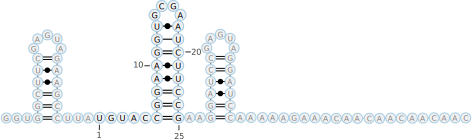
\includegraphics[width=0.6\textwidth]{/home/tsuname/Documents/lab/rhiju/papers/REEFFIT/hobartnerseq.png}
\caption{The full sequence of the Hobartner bistable RNA (the $hob_1$ structure is shown here). Auxiliary nucleotides are marked in gray.}.
\label{fig:hobartnerseq}
\end{figure}
%\begin{figure}[here]
%\includegraphics[width=0.9\textwidth]{/home/tsuname/Documents/lab/rhiju/papers/REEFFIT/reactivityhistograms.png}
%\caption{Histogram (blue bars) and cauchy approximation of the %difference in SHAPE reactivities from all M$^2$ experiments in %the RMDB. This distribution is used as a prior for the effects of %local perturbations induced by mutations.}.
%\label{fig:reactivityhistogramsfig}
%\end{figure}

% In silico benchmark table
\begin{table}[htbp]
\caption{Results for the \textit{in silico} simulated M$^2$ benchmark. }
\begin{tabular}{|l|p{0.5cm}|p{2cm}|p{2cm}|p{2cm}|p{2cm}|p{2cm}|}
\hline
Name & \multicolumn{1}{p{2cm}|}{Sequence length} & \multicolumn{1}{p{2cm}|}{Number of structures} & \multicolumn{1}{p{2cm}|}{Number of predicted structures} & \multicolumn{1}{p{2cm}|}{$\chi^2/df$} & \multicolumn{1}{p{2cm}|}{RMSEA} & \multicolumn{1}{p{2cm}|}{Percentage of weights correctly predicted} \\ \hline
RF01092;GP knot2 & 61 & 3 & 2 & 0.85 & 0.00 & 54.03 \\ \hline
RF01020;mir-572 & 56 & 7 & 2 & 1.22 & 0.06 & 81.58 \\ \hline
RF01313;HHBV epsilon & 57 & 7 & 2 & 1.21 & 0.06 & 100.00 \\ \hline
RF00066;U7 & 61 & 3 & 3 & 1.29 & 0.07 & 100.00 \\ \hline
RF01300;snoU49 & 58 & 3 & 3 & 1.33 & 0.08 & 66.10 \\ \hline
RF01139;sR2 & 55 & 3 & 2 & 1.50 & 0.10 & 89.29 \\ \hline
RF01274;sR45 & 55 & 4 & 2 & 1.08 & 0.04 & 100.00 \\ \hline
RF01297;sR40 & 61 & 4 & 2 & 1.56 & 0.10 & 100.00 \\ \hline
RF00555;L13 leader & 56 & 4 & 2 & 1.35 & 0.08 & 100.00 \\ \hline
RF00775;mir-432 & 53 & 3 & 3 & 1.17 & 0.06 & 56.17 \\ \hline
RF00173;Hairpin & 46 & 2 & 3 & 1.01 & 0.02 & 83.69 \\ \hline
RF00196;AMV RNA1 SL & 40 & 2 & 3 & 1.01 & 0.02 & 88.62 \\ \hline
RF00424;SCARNA16 & 53 & 3 & 2 & 1.30 & 0.08 & 87.04 \\ \hline
RF01383;GRIK4 3p UTR & 59 & 4 & 2 & 1.29 & 0.07 & 78.38 \\ \hline
RF00108;SNORD116 & 36 & 3 & 4 & 2.56 & 0.21 & 31.67 \\ \hline
RF00570;SNORD64 & 58 & 2 & 2 & 1.47 & 0.09 & 77.12 \\ \hline
RF01301;snoR4a & 53 & 2 & 2 & 1.18 & 0.06 & 81.48 \\ \hline
RF01125;sR4 & 58 & 4 & 4 & 1.61 & 0.10 & 93.64 \\ \hline
RF00436;UnaL2 & 32 & 3 & 2 & 1.41 & 0.12 & 36.36 \\ \hline
RF01151;snoU82P & 49 & 4 & 2 & 1.29 & 0.08 & 100.00 \\ \hline
\end{tabular}
\label{insilicobenchmark}
\end{table}
\begin{table}[htbp]
\caption{Primer sequences for the Hobartner bistable sequence PCR assembly}
\begin{tabular}{|l|p{20cm}|}
\hline
Primer 1 & TTCTAATACGACTCACTATAGGTGGC \\ \hline
Primer 2 & TCCGGTACATAAGGCTTCTACTCGAAGCCACCTATAGTGAGTCGT \\ \hline
Primer 3 & AGAAGCCTTATGTACCGGAAGGTGCGAATCTTCCGAAGGATCCGAGTAGGATCCAAA \\ \hline
Primer 4 & GTTGTTGTTGTTGTTTCTTTTTGGATCCTACTCGGATCCTTCGGAAGATTCGCA \\ \hline
\end{tabular}
\label{hobartnerprimers}
\end{table}

\end{document}